\documentclass[11pt]{article} %
\usepackage{times}
%
\usepackage[letterpaper, left=1in, right=1in, top=1in, bottom=1in]{geometry}

\usepackage[utf8]{inputenc} %
\usepackage[T1]{fontenc}    %

%
%
%
\usepackage{natbib}
%
\bibliographystyle{apalike} %
\bibpunct{(}{)}{;}{a}{,}{,}

\usepackage[utf8]{inputenc} %
\usepackage[T1]{fontenc}    %
\usepackage{hyperref}       %
\usepackage{url}            %
\usepackage{booktabs}       %
\usepackage{amsfonts}       %
\usepackage{nicefrac}       %
\usepackage{microtype}      %
\usepackage{xcolor}         %


%
\usepackage{graphicx}
\usepackage{subcaption}
\usepackage{amsmath,amssymb, amsthm}
\usepackage[capitalize, noabbrev]{cleveref}
\usepackage{multirow}
\usepackage{multicol}
\usepackage{mathtools}
\usepackage{ marvosym }
\usepackage{setspace}
\usepackage{textcomp}
\usepackage{authblk} 
\usepackage{bbm}
\usepackage{array}
\usepackage{algorithm}
\usepackage[noend]{algpseudocode}
\usepackage{rotating}
\usepackage[shortlabels]{enumitem}
\usepackage{tikz}
\usetikzlibrary{bayesnet}

\usepackage{apptools}
\usepackage[page, header]{appendix}
\usepackage{titletoc}


%
%

%
%
%
\theoremstyle{plain}
%
%
%
%
%
%
%
%
%

%
\newtheorem{theorem}{Theorem}
\newtheorem{proposition}{Proposition}
\newtheorem{lemma}{Lemma}
\newtheorem{corollary}{Corollary}
\theoremstyle{definition}
\newtheorem{definition}{Definition}
\newtheorem{assumption}{Assumption}
\theoremstyle{remark}
\newtheorem{remark}{Remark}



\let\oldReturn\Return
\renewcommand{\Return}{\State\oldReturn}
\newcommand{\bbeta}{\boldsymbol{\beta}}
\newcommand{\N}{\mbox{N}}
\newcommand{\PG}{\mbox{PG}}
\newcommand{\Ga}{\mbox{Ga}}
\newcommand{\Lo}{\mbox{Lo}}
\newcommand{\R}{\mathbb{R}}
\newcommand{\vnorm}[1]{\left|\left|#1\right|\right|}
\newcommand{\rejected}{\hat{\mathcal{S}}}
\newcommand{\nonnulls}{\mathcal{S}}
\newcommand{\nulls}{\bar{\mathcal{S}}}
\newcommand{\FPs}{V}
\newcommand{\qedwhite}{\hfill \ensuremath{\Box}}
\newcommand{\1}[1]{\mathbbm{1}\left[#1\right]}
\newcommand{\QED}{\hfill\qed}
\newcommand{\pr}{\textnormal{Pr}}
\newcommand{\indep}{\perp\!\!\!\!\perp} 
\DeclareMathOperator*{\ind}{1{\hskip -2.5 pt}\hbox{I}}  %
\newcommand{\Xcal}{\mathcal{X}}
\newcommand{\Ycal}{\mathcal{Y}}
\newcommand{\E}{\mathbb{E}}
\newcommand{\Z}{\mathbb{Z}}
\newcommand{\chris}[1]{{\color{blue}chris:\, #1}}
\newcommand{\Mcal}{\mathcal{M}}
\newcommand{\Ncal}{\mathcal{N}}
\newcommand{\Dcal}{\mathcal{D}}
\newcommand{\opt}{\operatorname{OPT}}

\newcommand{\bigCI}{\mathrel{\text{\scalebox{1.07}{$\perp\mkern-10mu\perp$}}}}
\newcommand{\argmin}{\operatorname{argmin}}

%
%
%
\usepackage[textsize=tiny]{todonotes}

\hypersetup{
  colorlinks   = true, %
  urlcolor     = blue, %
  linkcolor    = blue, %
  citecolor   = red %
}


\usepackage{authblk}

%
\title{\textbf{Treatment response as a latent variable}}
%
\author[1]{Christopher Tosh}
\author[2]{Boyuan Zhang}
\author[1]{Wesley Tansey}
\affil[1]{Memorial Sloan Kettering Cancer Center, New York, NY}
\affil[2]{Stanford University, Palo Alto, CA}


%
%
%
%
%

\begin{document}
\maketitle

{\def\thefootnote{}
\footnotetext{E-mail:
\texttt{christopher.j.tosh@gmail.com},\
\texttt{boyuanz@stanford.edu},\
\texttt{tanseyw@mskcc.org}}}

\vspace{-2em}
\begin{abstract}
  \begin{abstract}  
Test time scaling is currently one of the most active research areas that shows promise after training time scaling has reached its limits.
Deep-thinking (DT) models are a class of recurrent models that can perform easy-to-hard generalization by assigning more compute to harder test samples.
However, due to their inability to determine the complexity of a test sample, DT models have to use a large amount of computation for both easy and hard test samples.
Excessive test time computation is wasteful and can cause the ``overthinking'' problem where more test time computation leads to worse results.
In this paper, we introduce a test time training method for determining the optimal amount of computation needed for each sample during test time.
We also propose Conv-LiGRU, a novel recurrent architecture for efficient and robust visual reasoning. 
Extensive experiments demonstrate that Conv-LiGRU is more stable than DT, effectively mitigates the ``overthinking'' phenomenon, and achieves superior accuracy.
\end{abstract}  
\end{abstract}

\section{Introduction}
\label{sec:introduction}
The business processes of organizations are experiencing ever-increasing complexity due to the large amount of data, high number of users, and high-tech devices involved \cite{martin2021pmopportunitieschallenges, beerepoot2023biggestbpmproblems}. This complexity may cause business processes to deviate from normal control flow due to unforeseen and disruptive anomalies \cite{adams2023proceddsriftdetection}. These control-flow anomalies manifest as unknown, skipped, and wrongly-ordered activities in the traces of event logs monitored from the execution of business processes \cite{ko2023adsystematicreview}. For the sake of clarity, let us consider an illustrative example of such anomalies. Figure \ref{FP_ANOMALIES} shows a so-called event log footprint, which captures the control flow relations of four activities of a hypothetical event log. In particular, this footprint captures the control-flow relations between activities \texttt{a}, \texttt{b}, \texttt{c} and \texttt{d}. These are the causal ($\rightarrow$) relation, concurrent ($\parallel$) relation, and other ($\#$) relations such as exclusivity or non-local dependency \cite{aalst2022pmhandbook}. In addition, on the right are six traces, of which five exhibit skipped, wrongly-ordered and unknown control-flow anomalies. For example, $\langle$\texttt{a b d}$\rangle$ has a skipped activity, which is \texttt{c}. Because of this skipped activity, the control-flow relation \texttt{b}$\,\#\,$\texttt{d} is violated, since \texttt{d} directly follows \texttt{b} in the anomalous trace.
\begin{figure}[!t]
\centering
\includegraphics[width=0.9\columnwidth]{images/FP_ANOMALIES.png}
\caption{An example event log footprint with six traces, of which five exhibit control-flow anomalies.}
\label{FP_ANOMALIES}
\end{figure}

\subsection{Control-flow anomaly detection}
Control-flow anomaly detection techniques aim to characterize the normal control flow from event logs and verify whether these deviations occur in new event logs \cite{ko2023adsystematicreview}. To develop control-flow anomaly detection techniques, \revision{process mining} has seen widespread adoption owing to process discovery and \revision{conformance checking}. On the one hand, process discovery is a set of algorithms that encode control-flow relations as a set of model elements and constraints according to a given modeling formalism \cite{aalst2022pmhandbook}; hereafter, we refer to the Petri net, a widespread modeling formalism. On the other hand, \revision{conformance checking} is an explainable set of algorithms that allows linking any deviations with the reference Petri net and providing the fitness measure, namely a measure of how much the Petri net fits the new event log \cite{aalst2022pmhandbook}. Many control-flow anomaly detection techniques based on \revision{conformance checking} (hereafter, \revision{conformance checking}-based techniques) use the fitness measure to determine whether an event log is anomalous \cite{bezerra2009pmad, bezerra2013adlogspais, myers2018icsadpm, pecchia2020applicationfailuresanalysispm}. 

The scientific literature also includes many \revision{conformance checking}-independent techniques for control-flow anomaly detection that combine specific types of trace encodings with machine/deep learning \cite{ko2023adsystematicreview, tavares2023pmtraceencoding}. Whereas these techniques are very effective, their explainability is challenging due to both the type of trace encoding employed and the machine/deep learning model used \cite{rawal2022trustworthyaiadvances,li2023explainablead}. Hence, in the following, we focus on the shortcomings of \revision{conformance checking}-based techniques to investigate whether it is possible to support the development of competitive control-flow anomaly detection techniques while maintaining the explainable nature of \revision{conformance checking}.
\begin{figure}[!t]
\centering
\includegraphics[width=\columnwidth]{images/HIGH_LEVEL_VIEW.png}
\caption{A high-level view of the proposed framework for combining \revision{process mining}-based feature extraction with dimensionality reduction for control-flow anomaly detection.}
\label{HIGH_LEVEL_VIEW}
\end{figure}

\subsection{Shortcomings of \revision{conformance checking}-based techniques}
Unfortunately, the detection effectiveness of \revision{conformance checking}-based techniques is affected by noisy data and low-quality Petri nets, which may be due to human errors in the modeling process or representational bias of process discovery algorithms \cite{bezerra2013adlogspais, pecchia2020applicationfailuresanalysispm, aalst2016pm}. Specifically, on the one hand, noisy data may introduce infrequent and deceptive control-flow relations that may result in inconsistent fitness measures, whereas, on the other hand, checking event logs against a low-quality Petri net could lead to an unreliable distribution of fitness measures. Nonetheless, such Petri nets can still be used as references to obtain insightful information for \revision{process mining}-based feature extraction, supporting the development of competitive and explainable \revision{conformance checking}-based techniques for control-flow anomaly detection despite the problems above. For example, a few works outline that token-based \revision{conformance checking} can be used for \revision{process mining}-based feature extraction to build tabular data and develop effective \revision{conformance checking}-based techniques for control-flow anomaly detection \cite{singh2022lapmsh, debenedictis2023dtadiiot}. However, to the best of our knowledge, the scientific literature lacks a structured proposal for \revision{process mining}-based feature extraction using the state-of-the-art \revision{conformance checking} variant, namely alignment-based \revision{conformance checking}.

\subsection{Contributions}
We propose a novel \revision{process mining}-based feature extraction approach with alignment-based \revision{conformance checking}. This variant aligns the deviating control flow with a reference Petri net; the resulting alignment can be inspected to extract additional statistics such as the number of times a given activity caused mismatches \cite{aalst2022pmhandbook}. We integrate this approach into a flexible and explainable framework for developing techniques for control-flow anomaly detection. The framework combines \revision{process mining}-based feature extraction and dimensionality reduction to handle high-dimensional feature sets, achieve detection effectiveness, and support explainability. Notably, in addition to our proposed \revision{process mining}-based feature extraction approach, the framework allows employing other approaches, enabling a fair comparison of multiple \revision{conformance checking}-based and \revision{conformance checking}-independent techniques for control-flow anomaly detection. Figure \ref{HIGH_LEVEL_VIEW} shows a high-level view of the framework. Business processes are monitored, and event logs obtained from the database of information systems. Subsequently, \revision{process mining}-based feature extraction is applied to these event logs and tabular data input to dimensionality reduction to identify control-flow anomalies. We apply several \revision{conformance checking}-based and \revision{conformance checking}-independent framework techniques to publicly available datasets, simulated data of a case study from railways, and real-world data of a case study from healthcare. We show that the framework techniques implementing our approach outperform the baseline \revision{conformance checking}-based techniques while maintaining the explainable nature of \revision{conformance checking}.

In summary, the contributions of this paper are as follows.
\begin{itemize}
    \item{
        A novel \revision{process mining}-based feature extraction approach to support the development of competitive and explainable \revision{conformance checking}-based techniques for control-flow anomaly detection.
    }
    \item{
        A flexible and explainable framework for developing techniques for control-flow anomaly detection using \revision{process mining}-based feature extraction and dimensionality reduction.
    }
    \item{
        Application to synthetic and real-world datasets of several \revision{conformance checking}-based and \revision{conformance checking}-independent framework techniques, evaluating their detection effectiveness and explainability.
    }
\end{itemize}

The rest of the paper is organized as follows.
\begin{itemize}
    \item Section \ref{sec:related_work} reviews the existing techniques for control-flow anomaly detection, categorizing them into \revision{conformance checking}-based and \revision{conformance checking}-independent techniques.
    \item Section \ref{sec:abccfe} provides the preliminaries of \revision{process mining} to establish the notation used throughout the paper, and delves into the details of the proposed \revision{process mining}-based feature extraction approach with alignment-based \revision{conformance checking}.
    \item Section \ref{sec:framework} describes the framework for developing \revision{conformance checking}-based and \revision{conformance checking}-independent techniques for control-flow anomaly detection that combine \revision{process mining}-based feature extraction and dimensionality reduction.
    \item Section \ref{sec:evaluation} presents the experiments conducted with multiple framework and baseline techniques using data from publicly available datasets and case studies.
    \item Section \ref{sec:conclusions} draws the conclusions and presents future work.
\end{itemize}

\section{Background}\label{sec:backgrnd}

\subsection{Cold Start Latency and Mitigation Techniques}

Traditional FaaS platforms mitigate cold starts through snapshotting, lightweight virtualization, and warm-state management. Snapshot-based methods like \textbf{REAP} and \textbf{Catalyzer} reduce initialization time by preloading or restoring container states but require significant memory and I/O resources, limiting scalability~\cite{dong_catalyzer_2020, ustiugov_benchmarking_2021}. Lightweight virtualization solutions, such as \textbf{Firecracker} microVMs, achieve fast startup times with strong isolation but depend on robust infrastructure, making them less adaptable to fluctuating workloads~\cite{agache_firecracker_2020}. Warm-state management techniques like \textbf{Faa\$T}~\cite{romero_faa_2021} and \textbf{Kraken}~\cite{vivek_kraken_2021} keep frequently invoked containers ready, balancing readiness and cost efficiency under predictable workloads but incurring overhead when demand is erratic~\cite{romero_faa_2021, vivek_kraken_2021}. While these methods perform well in resource-rich cloud environments, their resource intensity challenges applicability in edge settings.

\subsubsection{Edge FaaS Perspective}

In edge environments, cold start mitigation emphasizes lightweight designs, resource sharing, and hybrid task distribution. Lightweight execution environments like unikernels~\cite{edward_sock_2018} and \textbf{Firecracker}~\cite{agache_firecracker_2020}, as used by \textbf{TinyFaaS}~\cite{pfandzelter_tinyfaas_2020}, minimize resource usage and initialization delays but require careful orchestration to avoid resource contention. Function co-location, demonstrated by \textbf{Photons}~\cite{v_dukic_photons_2020}, reduces redundant initializations by sharing runtime resources among related functions, though this complicates isolation in multi-tenant setups~\cite{v_dukic_photons_2020}. Hybrid offloading frameworks like \textbf{GeoFaaS}~\cite{malekabbasi_geofaas_2024} balance edge-cloud workloads by offloading latency-tolerant tasks to the cloud and reserving edge resources for real-time operations, requiring reliable connectivity and efficient task management. These edge-specific strategies address cold starts effectively but introduce challenges in scalability and orchestration.

\subsection{Predictive Scaling and Caching Techniques}

Efficient resource allocation is vital for maintaining low latency and high availability in serverless platforms. Predictive scaling and caching techniques dynamically provision resources and reduce cold start latency by leveraging workload prediction and state retention.
Traditional FaaS platforms use predictive scaling and caching to optimize resources, employing techniques (OFC, FaasCache) to reduce cold starts. However, these methods rely on centralized orchestration and workload predictability, limiting their effectiveness in dynamic, resource-constrained edge environments.



\subsubsection{Edge FaaS Perspective}

Edge FaaS platforms adapt predictive scaling and caching techniques to constrain resources and heterogeneous environments. \textbf{EDGE-Cache}~\cite{kim_delay-aware_2022} uses traffic profiling to selectively retain high-priority functions, reducing memory overhead while maintaining readiness for frequent requests. Hybrid frameworks like \textbf{GeoFaaS}~\cite{malekabbasi_geofaas_2024} implement distributed caching to balance resources between edge and cloud nodes, enabling low-latency processing for critical tasks while offloading less critical workloads. Machine learning methods, such as clustering-based workload predictors~\cite{gao_machine_2020} and GRU-based models~\cite{guo_applying_2018}, enhance resource provisioning in edge systems by efficiently forecasting workload spikes. These innovations effectively address cold start challenges in edge environments, though their dependency on accurate predictions and robust orchestration poses scalability challenges.

\subsection{Decentralized Orchestration, Function Placement, and Scheduling}

Efficient orchestration in serverless platforms involves workload distribution, resource optimization, and performance assurance. While traditional FaaS platforms rely on centralized control, edge environments require decentralized and adaptive strategies to address unique challenges such as resource constraints and heterogeneous hardware.



\subsubsection{Edge FaaS Perspective}

Edge FaaS platforms adopt decentralized and adaptive orchestration frameworks to meet the demands of resource-constrained environments. Systems like \textbf{Wukong} distribute scheduling across edge nodes, enhancing data locality and scalability while reducing network latency. Lightweight frameworks such as \textbf{OpenWhisk Lite}~\cite{kravchenko_kpavelopenwhisk-light_2024} optimize resource allocation by decentralizing scheduling policies, minimizing cold starts and latency in edge setups~\cite{benjamin_wukong_2020}. Hybrid solutions like \textbf{OpenFaaS}~\cite{noauthor_openfaasfaas_2024} and \textbf{EdgeMatrix}~\cite{shen_edgematrix_2023} combine edge-cloud orchestration to balance resource utilization, retaining latency-sensitive functions at the edge while offloading non-critical workloads to the cloud. While these approaches improve flexibility, they face challenges in maintaining coordination and ensuring consistent performance across distributed nodes.



\section{Model}
\label{sec:model}
Let $[N] = \{1, 2, \dots, N \}$ be a set of $N$ agents.
We examine an environment in which a system interacts with the agents over $T$ rounds.
Every round $t\leq T$ comprises $N$ \emph{sessions}, each session represents an encounter of the system with exactly one agent, and each agent interacts exactly once with the system every round.
I.e., in each round $t$ the agents arrive sequentially. 


\paragraph{Arrival order} The \emph{arrival order} of round $t$, denoted as $\ordv_t=(\ord_t(1),\dots, \ord_t(N))$, is an element from set of all permutations of $[N]$. Each entry $q$ in $\ordv_t$ is the index of the agent that arrives in the $q^{\text{th}}$ session of round $t$.
For example, if $\ord_t(1) = 2$, then agent $2$ arrives in the first session of round $t$.
Correspondingly, $\ord_t^{-1}(i)=q$ implies that agent $i$ arrives in the $q^{\text{th}}$ session of round $t$. 

As we demonstrate later, the arrival order has an immediate impact on agent rewards. We call the mechanism by which the arrival order is set \emph{arrival function} and denote it by $\ordname$. Throughout the paper, we consider several arrival functions such as the \emph{uniform arrival} function, denoted by $\uniord$, and the \emph{nudged arrival} $\sugord$; we introduce those formally in Sections~\ref{sec:uniform} and~\ref{sec:nudge}, respectively.

%We elaborate more on this concept in Section~\ref{sec: arrival}.


\paragraph{Arms} We consider a set of $K \geq 2$ arms, $A = \{a_1, \ldots, a_K\}$. The reward of arm $a_i$ in round $t$ is a random variable $X_i^t \sim \mathcal{D}^t_i$, where the rewards $(X_i^t)_{i,t}$ are mutually independent and bounded within the interval $[0,1]$. The reward distribution $\mathcal{D}^t_i$ of arm $a_i$, $i\in [K]$ at round $t\in T$ is assumed to be non-stationary but independent across arms and rounds. We denote the realized reward of arm $a_i$ in round $t$ by $x_i^t$. We assume \emph{reward consistency}, meaning that rewards may vary between rounds but remain constant within the sessions of a single round. Specifically, if an arm $a_i$ is selected multiple times during round~$t$, each selection yields the same reward $x_i^t$, where the superscript $t$ indicates its dependence on the round rather than the session. This consistency enables the system to leverage information obtained from earlier sessions to make more informed decisions in later sessions within the same round. We provide further details on this principle in Subsection~\ref{subsec:information}.


\paragraph{Algorithms} An algorithm is a mapping from histories to actions. We typically expect algorithms to maximize some aggregated agent metric like social welfare. Let $\mathcal H^{t,q}$ denote the information observed during all sessions of rounds $1$ to $t-1$ and sessions $1$ to $q-1$ in round $t$.  The history $\mathcal H^{t,q}$ is an element from $(A \times [0,1])^{(t-1) \cdot N +q-1}$, consisting of pairs of the form (pulled arm, realized reward). Notice that we restrict our attention to \emph{anonymous} algorithms, i.e., algorithms that do not distinguish between agents based on their identities. Instead, they only respond to the history of arms pulled and rewards observed, without conditioning on which specific agent performed each action.
%In the most general case, algorithms make decisions at session $q$ of round $t$  based on the entire history $\mathcal H^{t,q}$ and the index of the arriving agent $\ord_t(q)$. %Furthermore, we sometimes assume that algorithms have Bayesian information, i.e., algorithms are aware of the distributions $(\mathcal D_i)^K_{i=1}$. 
Furthermore, we sometimes assume that algorithms have Bayesian information, meaning they are aware of the reward distributions $(\mathcal{D}^t_i)_{i,t}$. If such an assumption is required to derive a result, we make it explicit. %Otherwise, we do not assume any additional knowledge about the algorithm’s information. %This distinction allows us to analyze both general algorithms without prior distributional knowledge and specialized algorithms that leverage Bayesian information.


\paragraph{Rewards} Let $\rt{i}$ denote the reward received by agent $i \in [N]$ at round $t$, and let $\Rt{i}$ denote her cumulative reward at the end of round $t$, i.e., $\Rt{i} = \sum_{\tau=1}^{t}{r^{\tau}_{i}}$. We further denote the \emph{social welfare} as the sum of the rewards all agents receive after $T$ rounds. Formally, $\sw=\sum^{N}_{i=1}{R^T_i}$. We emphasize that social welfare is independent of the arrival order. 


\paragraph{Envy}
We denote by $\adift{i}{j}$ the reward discrepancy of agents $i$ and $j$ in round $t$; namely, $\adift{i}{j}= \rt{i} - \rt{j}$. %We call this term \omer{name??} reward discrepancy in round $t$. 
The (cumulative) \emph{envy} between two agents at round $t$ is the difference in their cumulative rewards. Formally, $\env_{i,j}^t= \Rt{i} - \Rt{j}$ is the envy after $t$ rounds between agent $i$ and $j$. We can also formulate envy as the sum of reward discrepancies, $\env_{i,j}^t= \sum^{t}_{\tau=1}{\adif{i}{j}^\tau}$. Notice that envy is a signed quantity and can be either positive or negative. Specifically, if $\env_{i,j}^t < 0$, we say that agent $i$ envies agent $j$, and if $\env_{i,j}^t > 0$, agent $j$ envies agent $i$. The main goal of this paper is to investigate the behavior of the \emph{maximal envy}, defined as
\[
\env^t = \max_{i,j \in [N]} \env^t_{i,j}.
\]
For clarity, the term \emph{envy} will refer to the maximal envy.\footnote{ We address alternative definitions of envy in Section~\ref{sec:discussion}.} % Envy can also be defined in alternative ways, such as by averaging pairwise envy across all agents. We address average envy in Section~\ref{sec:avg_envy}.}
Note that $\env_{i,j}^t$ are random variables that depend on the decision-making algorithm, realized rewards, and the arrival order, and therefore, so is $\env^t$. If a result we obtain regarding envy depends on the arrival order $\ordname$, we write $\env^t(\ordname)$. Similarly, to ease notation, if $\ordname$ can be understood from the context, it is omitted.



\paragraph{Further Notation} We use the subscript $(q)$ to address elements of the $q^{\text{th}}$ session, for $q\in [N]$.
That is, we use the notation $\rt{(q)}$ to denote the reward granted to the agent that arrives in the $q^{\text{th}}$ session of round $t$ and $\Rt{(q)}$ to denote her cumulative reward. %Additionally, we introduce the notation $\at{(q)}$ to denote the arm pulled in that session.
Correspondingly, $\sdift{q}{w} = \rt{(q)} - \rt{(w)}$ is the reward discrepancy of the agents arriving in the $q^{\text{th}}$ and $w^{\text{th}}$ sessions of round $t$, respectively. 
To distinguish agents, arms, sessions and rounds, we use the letters $i,j$ to mark agents and arms, $q,w$ for sessions, and $t,\tau$ for rounds.


\subsection{Example}
\label{sec: example}
To illustrate the proposed setting and notation, we present the following example, which serves as a running example throughout the paper.

\begin{table}[t]
\centering
\begin{tabular}{|c|c|c|c|}
\hline
$t$ (round) & $\ordv_t$ (arrival order) & $x_1^t$ & $x_2^t$ \\ \hline
1           & 2, 1                     & 0.6     & 0.92    \\ \hline
2           & 1, 2                     & 0.48    & 0.1     \\ \hline
3           & 2, 1                     & 0.15    & 0.8     \\ \hline
\end{tabular}
\caption{
    Data for Example~\ref{example 1}.
}
\label{tbl: example}
\end{table}

\begin{algorithm}[t]
\caption{Algorithm for Example~\ref{example 1}}
\label{alguni}
\DontPrintSemicolon 
\For{round $t = 1$ to $T$}{
    pull $a_{1}$ in the first session\label{alguniexample: first}\\
    \lIf{$x^t_1 \geq \frac{1}{2}$}{pull $a_{1}$ again in second session \label{alguniexample: pulling a again}}
    \lElse{pull $a_{2}$ in second session \label{alguniexample: sopt else}}
}
\end{algorithm}


\begin{example}\label{example 1}
We consider $K=2$ uniform arms, $X_1,X_2 \sim \uni{0,1}$, and $N=2$ for some $T\geq 3$. We shall assume arm decision are made by Algorithm~\ref{alguni}: In the first session, the algorithm pulls $a_1$; if it yields a reward greater than $\nicefrac{1}{2}$, the algorithm pulls it again in the second session (the ``if'' clause). Otherwise, it pulls $a_2$.



We further assume that the arrival orders and rewards are as specified in Table~\ref{tbl: example}. Specifically, agent 2 arrives in the first session of round $t=1$, and pulling arm $a_2$ in this round would yield a reward of $x^1_2 = 0.92$. Importantly, \emph{this information is not available to the decision-making algorithm in advance} and is only revealed when or if the corresponding arms are pulled.




In the first round, $\boldsymbol{\eta}^1 = \left(2,1\right)$; thus, agent 2 arrives in the first session.
The algorithm pulls arm $a_1$, which means, $a^1_{(1)} = a_1$, and the agent receives $r_{2}^1=r_{(1)}^1=x_1^1=0.6$.
Later that round, in the second session, agent 1 arrives, and the algorithm pulls the same arm again since $x^1_1 = 0.6 \geq \nicefrac{1}{2}$ due to the ``if'' clause.
I.e., $a^1_{(2)} = a_1$ and $r_{1}^1 = r_{(2)}^1 = x_1^1 = 0.6$.
Even though the realized reward of arm $a_2$ in that round is higher ($0.92$), the algorithm is not aware of that value.
At the end of the first round, $R^1_1 = R^1_{(2)} = R^1_2 = R^1_{(1)} = 0.6$. The reward discrepancy is thus $\adif{1}{2}^1 = \adif{2}{1}^1= \sdif{2}{1}^1 = 0.6 - 0.6 =0$. 



In the second round, agent 1 arrives first, followed by agent 2.
Firstly, the algorithm pulls arm $a_1$ and agent 1 receives a reward of $r_{1}^2 = r_{(1)}^2 = x_1^2 = 0.48$.
Because the reward is lower than $\nicefrac{1}{2}$, in the second session the algorithm pulls the other arm ($a^2_{(2)} = a_2$), granting agent 2 a reward of $r_{2}^2 = r_{(2)}^2 = x_2^2 = 0.1$.
At the end of the second round, $R^2_1 = R^2_{(1)} = 0.6 + 0.48 = 1.08$ and $R^2_2 = R^2_{(2)} = 0.6 + 0.1 = 0.7$. Furthermore, $\sdif{2}{1}^2 = \adif{2}{1}^2 = r^2_{2} - r^2_{1} = 0.1 - 0.48 = -0.38$.

In the third and final round, agent 2 arrives first again, and receives a reward  of $0.15$ from $a_1$. When agent 1 arrives in the second session, the algorithm pulls arm $a_2$, and she receives a reward of $0.8$. As for the reward discrepancy, $\sdif{2}{1}^3 = \adif{2}{1}^3 = r^3_{2} - r^3_{1} = 0.15 - 0.8 = -0.75$. 

Finally, agent 1 has a cumulative reward of $R^3_1 = R^3_{(2)} = 0.6 + 0.48 + 0.8 = 1.88$, whereas agent~2 has a cumulative reward of $R^3_2 = R^3_{(1)} = 0.6 + 0.1 + 0.15 = 0.85$. In terms of envy, $\env^1_{1,2}= \adif{1}{2}^1 =0$, $\env^2_{1,2}=\adif{1}{2}^1+\adif{1}{2}^2= 0.38$, and $\env^3_{1,2} = -\env^3_{2,1} = R^3_1-R^3_2 = 1.88-0.85 = 1.03$, and consequently the envy in round 3 is $\env^3 = 1.03$.
\end{example}


\subsection{Information Exploitation}
\label{subsec:information}

In this subsection, we explain how algorithms can exploit intra-round information.
Since rewards are consistent in the sessions of each round, acquiring information in each session can be used to increase the reward of the following sessions.
In other words, the earlier sessions can be used for exploration, and we generally expect agents arriving in later sessions to receive higher rewards.
Taken to the extreme, an agent that arrives after all arms have been pulled could potentially obtain the highest reward of that round, depending on how the algorithm operates.

To further demonstrate the advantage of late arrival, we reconsider Example~\ref{example 1} and Algorithm~\ref{alguni}. 
The expected reward for the agent in the first session of round $t$ is $\E{\rt{(1)}}=\mu_1=\frac{1}{2}$, yet the expected reward of the agent in the second session is
\begin{align*}
\E{\rt{(2)}}=\E{\rt{(2)}\mid X^t_1 \geq \frac{1}{2} }\prb{X^t_1 \geq \frac{1}{2}} + \E{\rt{(2)}\mid X^t_1 < \frac{1}{2} }\prb{X^t_1 < \frac{1}{2}};
\end{align*}
thus, $\E{\rt{(2)}} =\E{X^t_1\mid X^t_1 \geq \frac{1}{2} }\cdot \frac{1}{2} + \mu_2\cdot\frac{1}{2} = \frac{5}{8}$.
Consequently, the expected welfare per round is $\E{\rt{(1)}+\rt{(2)}}=1+\frac{1}{8}$, and the benefit of arriving in the second session of any round $t$ is $\E{\rt{(2)} - \rt{(1)}} = \frac{1}{8}$. This gap creates envy over time, which we aim to measure and understand.
%This discrepancy generates envy over time, and our paper aims to better understand it.
\subsection{Socially Optimal Algorithms}
\label{sec: sw}
Since our model is novel, particularly in its focus on the reward consistency element, studying social welfare maximizing algorithms represents an important extension of our work. While the primary focus of this paper is to analyze envy under minimal assumptions about algorithmic operations, we also make progress in the direction of social welfare optimization. See more details in Section~\ref{sec:discussion}.%Due to space limitations, we defer the discussion on socially optimal algorithms to  \ifnum\Includeappendix=0{the appendix}\else{Section~\ref{appendix:sociallyopt}}\fi.




% Since our model is novel and specifically the reward consistency element, it might be interesting to study social welfare optimization. While the main focus of our paper is to study envy under minimal assumptions on how the algorithm operates, we take steps toward this direction as well. Due to space limitations, we defer the discussion on socially optimal algorithms to  \ifnum\Includeappendix=0{the appendix}\else{Section~\ref{appendix:sociallyopt}}\fi.  We devise a socially optimal algorithm for the two-agent case, offer efficient and optimal algorithms for special cases of $N>2$ agents, and an inefficient and approximately optimal algorithm for any instance with $N>2$. Moreover, we address the welfare-envy tradeoff in Section~\ref{sec:extensions}.


% Social welfare, unlike envy, is entirely independent of the arrival order. While the main focus of our paper is to study envy under minimal assumptions on how the algorithm operates, socially optimal algorithms might also be of interest. Due to space limitations, we defer the discussion on socially optimal algorithms to  \ifnum\Includeappendix=0{the appendix}\else{Section~\ref{appendix:sociallyopt}}\fi. We devise a socially optimal algorithm for the two-agent case, offer efficient and optimal algorithms for special cases of $N>2$ agents, and an inefficient and approximately optimal algorithm for any instance with $N>2$. %Furthermore, we treat the welfare-envy tradeoff of the special case of Example~\ref{example 1}.





%
\section{A semi-parametric additive errors model}
\label{sec:additive}
In the additive errors (AE) regime, we model $y$ as a deterministic function plus mean zero i.i.d. noise,
\begin{equation}
\label{eqn:additive_errors}
\begin{aligned}
(y \mid x, h=0) &=& \mu_0(x) + \epsilon  & &\\
(y \mid x, h=1) &=& \mu_1(x) + \epsilon &=& \mu_0(x) + \tau(x) + \epsilon\\
\epsilon &\sim& g(\epsilon)\,, && \mathbb{E}[\epsilon] = 0  \, , 
\end{aligned}
\end{equation}
where $\tau(x) = \mu_1(x) - \mu_0(x)$ is the expected difference in outcome between the responder and non-responder models. \cref{eqn:additive_errors} is common in many causal inference setups, particularly when estimating the conditional average treatment effect \citep[cf.][]{hahn:etal:2017:bcf,wager:athey:2018:causal-forests}. This setting can be thought of as a conditionally semi-parametric model. Conditioned on covariates $x$, the model consists of the parameters $\mu_0(x), \mu_1(x)$ and the infinite-dimensional model for the noise $\epsilon$. The AE model is strictly more flexible than a parametric model with a location parameter. Despite the added flexibility, we can show that this model is identifiable, meaning we can directly estimate the underlying parameters.

\begin{theorem}
\label{thm:additive-identify}
The model in \cref{eqn:additive_errors} is identifiable at every $x$.
\end{theorem}

The upshot to \cref{thm:additive-identify} is that we can fit a semi-parametric model to \cref{eqn:additive_errors} and use the resulting model to test the hypothesis $H_0: \mathbb{E}[y - \mu_0(x)] = 0$. 
We can also directly interpret $\tau(x)$ as the CARE for a sample with covariates $x$. 
Additionally, after fitting a semi-parametric model to \cref{eqn:additive_errors}, we can also recover the ERPF from our estimate of $\pi$.


To fit a model to \cref{eqn:additive_errors}, we follow a stagewise procedure. First, we fit a nonparametric regression function $\hat{\mu}_0(x)$ to the expected outcomes for the untreated population. Next, we use a nonparametric density estimator to marginally model the residual error distribution $\hat{g}$ of $y - \hat{\mu}_0(x)$ on the untreated population. Finally, we use an EM algorithm to fit nonparametric regression functions $\hat{\pi}$ and $\hat{\mu}_1$ for the prior and responder model, respectively, on the treated population, utilizing $\hat{g}$ and $\hat{\mu}_0$. The remainder of this section details the above approach.


\subsection{Estimating the non-response distribution}
\label{subsec:additive:null}
We model $\hat{\mu}_0$ using kernel ridge regression with a radial basis function kernel, and we fit it on the untreated population, using generalized cross-validation to select the bandwidth and regularization parameters~\citep{golub:etal:1979:gen-cv}. After fitting $\hat{\mu}_0$, we compute the leave-one-out predictions for each point in the untreated population, which can be calculated efficiently in closed form. We use these conditional expectations to estimate the residual noise distribution $g$. Cross-validation generally produces a biased-upward estimate of the true error distribution \citep{efron:gong:1983:leisurely-cv}. By overestimating the tails of the residual distribution, we conservatively bias the posterior probability of a response downward and the local FDR estimates upward.

We estimate the distribution of residuals $\hat{g}$ nonparametrically. We use predictive recursion \citep{martin:tokdar:2009:predictive-recursion} for its good rates of convergence and strong performance in other two-groups models \citep{scott:etal:2014:fdr-regression,tansey:etal:2018:fdr-smoothing}.
We choose the bandwidth by maximizing the predictive recursion marginal likelihood (PRML) \citep{martin:tokdar:2011:pr-marginal-likelihood}. This yields a tighter fit to the data and makes the density estimation routine fully auto-tuned and data-adaptive.

\subsection{Estimating the prior and response distributions}
\label{subsec:additive:alternative}
With $\hat{g}$ and $\hat{\mu}_0$ in hand, we form an estimate of the alternative distribution for the treated population. Specifically, we model each member of the treatment population as arising from the mixture model
\begin{equation}
\label{eqn:residual_mixture}
(y \mid x, t=1) \sim (1-\pi(x)) \hat{g}(y - \hat{\mu}_0(x)) + \pi(x) \hat{g}(y - \mu_1(x)) \, .
\end{equation}
We fit \cref{eqn:residual_mixture} via expectation-maximization with the following steps.

\paragraph{E-step.} Fix the estimates $\hat{\pi}$ and $\hat{\mu}_1$. Calculate the expected posterior probability of each data point coming from $\hat{g}(y - \mu_0(x))$,
\begin{equation*}
\label{eqn:additive_e_step}
\hat{w}_i = \frac{(1-\hat{\pi}(x_i)) \hat{g}(y_i - \hat{\mu}_0(x))}{(1-\hat{\pi}(x_i)) \hat{g}(y_i - \hat{\mu}_0(x)) + \hat{\pi}(x_i) \hat{g}(y_i - \hat{\mu}_1(x))} \, .
\end{equation*}
The posterior expectations $\hat{w}$ then serve as weights in the M-step.

\paragraph{M-step.} Fixing the weights $\hat{w}$, the optimization problem is separable in $\mu_1$ and $\pi$,
\begin{equation*}
\label{eqn:additive_m_step}
\begin{aligned}
\hat{\pi} &= \underset{\pi}{\text{argmax}} \sum_{i=1}^n \left[ \hat{w}_i \log(1-\pi(x_i)) + (1-\hat{w}_i) \log(\pi(x_i)) \right] \\
\hat{\mu}_1 &= \underset{\mu_1}{\text{argmax}} \sum_{i=1}^n (1-\hat{w}_i) \log(\hat{g}(y_i - \mu_1(x_i))) \, .
\end{aligned}
\end{equation*}
Both $\hat{\mu}_1$ and $\hat{\pi}$ (in logit-space) are encoded as linear models on top of random Fourier features, which approximate the full kernelized models and can be fit using gradient-based methods~\citep{rahimi:recht:2007:random-fourier-features}. The bandwidth parameters are selected using $k$-fold cross validation, and final predictions for the treated population are made on each held-out fold.

\subsection{Selecting responders}
\label{subsec:method:selection}
The final E-step estimate $\hat{w}$ has the appeal of both frequentist and Bayesian interpretations. Frequentists can interpret $\hat{w}\times 100$ as a local false discovery rate. Bayesians can interpret $1-\hat{w}$ as a posterior probability of treatment response. To select responders, we order the $\hat{w}$ values in ascending order and select the largest subset $\hat{S} \subset [n]$ such that $\frac{1}{|\hat{S}|} \sum_{i \in \hat{S}} \hat{w}_i \leq \alpha$, for a target $\alpha$-level FDR. While FDR control is guaranteed if we have the true posteriors~\citep{efron2012}, in practice with finite samples we will have some estimation error. Under some regularity assumptions, we can show that that excess FDR can be bounded above as a function of the estimation error.

\begin{assumption}
\label{assump:add-assumptions}
Let $\epsilon, \lambda, L, U > 0$ be given. Suppose the following holds for all $i=1,\ldots, n$:
\begin{itemize}
    \item[(i)] $g$ is $\lambda$-Lipschitz and bounded above by $U$,
    \item[(ii)] $(1-\pi(x_i))g(y_i - \mu_0(x_i)) + \pi(x_i) g(y_i - \mu_1(x_i)) \geq L$,
    \item [(iii)] $|\pi(x_i) - \hat{\pi}(x_i)|, |\mu_0(x_i) - \hat{\mu}_0(x_i)|, |\mu_1(x_i) - \hat{\mu}_1(x_i)| \leq \epsilon$, and
    \item[(iv)] $|g(y) - \hat{g}(y)| \leq \epsilon$ for all $y \in \R$.
\end{itemize}
\end{assumption}
Assumptions (i) and (ii) require the residual distribution and the treatment distributions to be well-behaved and are similar to standard assumptions made in the density estimation literature. Assumptions (iii) and (iv) reflect the quality of the estimators. This approximation error linearly translates to FDR.
\begin{theorem}
\label{thm:additive-fdr}
Suppose \cref{assump:add-assumptions} holds. If $\epsilon \leq \min \{1, L/4(U+2(\lambda + 1)) \}$, then the procedure outlined above results in FDR bounded by $\alpha + \delta$, where $\delta = \frac{2U(U+2(\lambda + 1))}{L^2} \epsilon$.
\end{theorem}
Thus, so long as we are reasonably accurate in our estimates, the realized FDR will be close to the target FDR.
Further, the power of the procedure can also be bounded from below as a function of the error, where the power of a procedure that selects a subset $V \subset \{ i \in [n]: t_i=1 \}$ is the expected fraction of individuals with $h_i = 1$, i.e. $\E\left[ \frac{1}{n} \sum_{i \in V} \ind[h_i = 1] \right]$. As in the FDR bound, approximation error also translates linearly to power.
\begin{theorem}
\label{thm:additive-power}
Suppose \cref{assump:add-assumptions} holds. The power of the procedure is bounded below by 
\[ \frac{1-\alpha - \delta}{1-\alpha + \delta + 1/(n_{\opt}(\alpha - \delta) +1)} \opt(\alpha - \delta), \]
where $\opt(\beta)$ is the power of the Bayes' optimal procedure that achieves FDR bounded above by $\beta$, $n_{\opt}(\beta)$ is the corresponding number of selections, and $\delta = \frac{2U(U+2(\lambda + 1))}{L^2} \epsilon$.
\end{theorem}
The number of selections plays a role in the quality of the power approximation in \cref{thm:additive-power}. This factor arises due to the discrete nature of the selection problem and the fact that it may not be possible to choose a subset with predicted FDR exactly equal to some quantity. However, as the number of optimal selections increases, the approximation ratio tends to $(1-\alpha-\delta)/(1-\alpha + \delta)$. Thus, with small model error, the selection procedure tends toward optimal power.



\section{Causal two-groups with nonparametric models}
\label{sec:kernel_generalized}
The additivity assumption in \cref{eqn:additive_errors} is often violated in practice. For instance, \citet{efron:feldman:1991:compliance} observed that higher rates of compliance were associated with increased variability in outcomes for both the treatment and control groups. Further, the increase in variance differed between treatment and control groups, suggesting that the error models for the two distributions $f_0$ and $f_1$ were different in the study.

Here, we propose a generalized empirical Bayes procedure for estimation in the causal two-groups model. The goal is to be maximally flexible to the true data generating model. As such, we remove the assumption of additive errors and instead directly model the outcome distributions in \cref{eqn:two_groups}. The starting point for this approach is the following result.
\begin{lemma}
\label{lem:conservative-pi}
Suppose the generative model from \cref{eqn:two_groups} induces treated distribution $f_t(y \mid x)$ and untreated distribution $f_0(y \mid x)$. Then for any $x$, we have
\[ \pi(x) \geq \pi^\star(x) := 1 - \min_y \frac{f_t(y \mid x)}{f_0(y \mid x)}. \]
Moreover, for any function $\pi$ satisfying $\pi(x) \in [\pi^\star(x), 1]$ for all $x$, there is an alternative distribution $f^\pi_1$ such that
\begin{align*}
f_t(y \mid x) &= (1-\pi(x)) f_0(y \mid x) + \pi(x) f^\pi_1(y \mid x).
\end{align*}
\end{lemma}
The implication of \cref{lem:conservative-pi} is that given the observed null and treatment distributions, one can compute the most conservative mixing function, $\pi^\star$, by minimizing their ratio. This leads to a valid test for an observation $(x,y)$ that controls the Type I error rate:
\begin{equation}
\label{eqn:general-bayes-test}
    \hat{h}_{\text{Bayes}} = \ind\left[ \frac{(1 -\pi^\star(x)) f_0(y \mid x) }{\pr(y \mid x, t=1)} \leq \alpha  \right] .
\end{equation}
Thus, empirical Bayesian testing in the fully general causal two-groups model can be reduced to finding suitable estimates of $f_0$ and $f_t$.

\subsection{Estimating the non-response and treatment distributions}
\label{subsec:kernel_generalized:estimation}
We take a nonparametric approach to approximating $f_0$ and $f_t$, using a $k$ nearest-neighbor version of the Rosenblatt kernel conditional density estimator~\citep{holmes:etal:2007:kernel-density-estimation,rosenblatt:1969:kernel-density-estimation}. That is, we approximate $f_t$ as
\[ \hat{f_t}(y \mid x ) = \frac{\sum_{i=1}^k K_{h_1}(x \mid x_{j_{x,1,i}})K_{h_2}(y \mid y_{j_{x,1,i}})}{\sum_{i=1}^k K_{h_1}(x \mid x_{j_{x,1,i}})}, \]
where $K_h$ is a probability kernel with bandwidth parameter $h>0$ and $j_{x,t,i}$ is the index of the $i$-th nearest neighbor of $x$ with treatment value $t$ in the dataset. $\hat{f_0}$ is constructed identically, substituting $j_{x,0,i}$ for $j_{x,1,i}$. The bandwidth parameters $h_1, h_2$ and number of neighbors $k$ are selected via leave-one-out cross validation.


\subsection{Selecting responders}
\label{subsec:kernel_generalized:estimation}
The test in \cref{eqn:general-bayes-test} relies on ratios of densities, making it sensitive to errors in our estimates. To address this issue, we use bootstrap sampling to create a population of conditional densities and estimate the ratios by using upper/lower quantiles to produce conservative ratio estimates. The final null posterior probability estimate for observation $x_i, y_i$ is given by
\begin{align}
\hat{w}_i = \frac{\hat{f}_{0,1-q}(y_i \mid x_i) }{\hat{f}_{t,q}(y_i \mid x_i)} \cdot \min_{y} \frac{\hat{f}_{t,1-q}(y \mid x_i)}{\hat{f}_{0,q}(y \mid x_i)},
\label{eqn:generalized_w_estimate}
\end{align}
where $\hat{f}_{t,q}(y\mid x)$ is the $q$-th quantile (under the bootstrap distribution) of the conditional treatment density of $y$ given $x$. Similarly, $\hat{f}_{0,q}(y\mid x)$ is the $q$-th quantile of the conditional untreated distribution. As in the additive case, we can sort the $\hat{w}$ values and select the largest subset such that their average value is below $\alpha$. The following result shows that when the conditional distributions are estimated accurately enough, the procedure results in proper FDR control.

\begin{theorem}
\label{thm:general-fdr}
Let $\epsilon, L, U > 0$ be given. Suppose the following holds for all $i=1,\ldots, n$ and $y \in \R$:
\begin{itemize}
    \item[(i)] $L \leq f_t(y \mid x_i), f_0(y \mid x_i) \leq U$,
    \item [(ii)] $|f_t(y \mid x_i) - \hat{f}_t(y \mid x_i)| \leq \epsilon$, and
    \item[(iii)] $|f_0(y \mid x_i) - \hat{f}_0(y \mid x_i)| \leq \epsilon$.
\end{itemize}
If $\epsilon \leq \min(1, L/2)$, then the procedure outlined above results in FDR bounded by $\alpha + \delta$, where $\delta = \frac{8U}{L^2} \left( 1 + \frac{12U}{L^2}\right)\epsilon$. 
Moreover, the power of the procedure is bounded below by 
\[ \frac{1-\alpha - \delta}{1-\alpha + \delta + 1/(n_{\opt}(\alpha - \delta) +1)} \opt(\alpha - \delta), \]
where $\opt(\beta)$ is the power of the Bayes' optimal procedure under the conservative prior of \Cref{lem:conservative-pi} that achieves FDR bounded above by $\beta$, and $n_{\opt}(\beta)$ is the corresponding number of selections.
\end{theorem}


We further control FDR with an empirical estimate of the FDR, calculated by performing the above selection procedure on both the treated and untreated populations over a grid of nominal FDR values $\alpha_1 < \alpha_2 < \cdots < \alpha_m$, and taking $e_k$ to be the ratio of the number of untreated selected at level $\alpha_k$ over the number of treated selected at level $\alpha_k$. Selection at level $\alpha$ proceeds by finding the largest $\alpha_k \leq \alpha$ such that $e_k \leq \alpha_k$ and selecting at level $\alpha_k$. We call this procedure \emph{empirical control}.

\subsection{Estimand intervals}
\label{subsec:kernel_generalized:estimands}
Beyond providing a test with valid FDR, \cref{lem:conservative-pi} also provides insights on the range of possible effects that can be ascribed to a possible response distribution. Specifically, because the model is not identifiable, one can not estimate a single latent response effect. Rather, \cref{lem:conservative-pi} implies that there is an \emph{interval} of feasible effects as summed up by the following corollary.

\begin{corollary}
\label{corr:np-ite}
Let $f_0(y \mid x)$, $f_t(y \mid x)$, and $\pi^\star(x)$ be as defined in \cref{lem:conservative-pi}. If $f_1$ is a valid responder distribution in \cref{eqn:two_groups}, we must have 
\[ \E_{f_1}[Y|X=x] \in \left[\mu_t(x),  \mu_1^\star(x) \right] \cup \left[\mu_1^\star(x), \mu_t(x) \right], \]
where 
\begin{align*}
\mu_t(x) = \E[Y | X=x, T=1], 
\mu_0(x) = \E[Y | X=x, T=0], \text{ and }
\mu_1^\star(x) = \frac{1}{\pi^\star(x)}(\mu_t(x) - \mu_0(x))  - \mu_0(x).
\end{align*}
Moreover, for any $v \in \left[\mu_t(x),  \mu_1^\star(x)\right] \cup \left[\mu_1^\star(x), \mu_t(x) \right]$, there is a valid responder distribution $f_1$ such that $\E_{f_1}[Y|X=x] = v$.
\end{corollary}
In the above statement, we have used the convention that $[a,b]$ is empty whenever $b<a$. Thus, for any individual $x$, the CARE lies in an interval that is bounded on one side by the CATE value $\mu_t(x) - \mu_0(x)$ and on the other side by the extremal CARE value of $\mu_1^\star(x) - \mu_0(x)$.

\begin{figure*}
\centering
\includegraphics[width=.95\textwidth]{plots/gradient.pdf}
\caption{Nonparametric C2G example. \emph{Left:} An example of a non-responder density (black), a treatment density (red), an extremal responder density (blue), and the range of feasible responder densities (gradient). \emph{Right:} Each feasible responder density has an associated prior probability and CARE value.}
\label{fig:npc2g-example}
\end{figure*}

\cref{fig:npc2g-example} shows an example of the nonparametric C2G setup: the control density, the treatment density, and the range of feasible responder densities. We see that at one end of the scale, the treatment density itself is a feasible alternative, with an associated prior probability $\pi(x) = 1$ and induced CARE equal to the CATE. On the other end of the scale, there is an extremal responder density with a smaller associated prior probability ($\pi(x) = \pi^\star(x)$) and larger CARE value. The relationship between these quantities is that as the prior probability grows towards one, the CARE shrinks towards the CATE, reflecting the fact that the associated responder distribution must also shrink towards the treatment distribution itself.





\section{Robustness against unmeasured confounding}
\label{sec:confounding}

\begin{figure*}[t]
\centering
\begin{subfigure}{0.22\linewidth}
\centering
\scalebox{0.7}{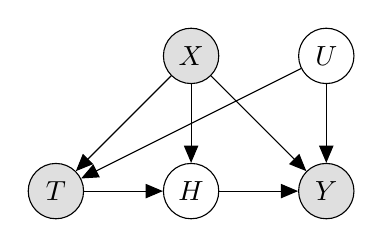
\begin{tikzpicture}

  %
  \node[obs, ]                               (x) {$X$};
  \node[latent, below=of x]                (h) {$H$};
  \node[obs, left=of h]                   (t) {$T$};
  \node[obs, right=of h]                   (y) {$Y$};
  \node[latent, right=of x]                 (u) {$U$};

  %
  \edge {x} {t} ; %
  \edge {x} {h}  ; %
  \edge {x} {y}  ; %
  \edge {t} {h}  ; %
  \edge {h} {y}  ; %
  \edge {u} {t}  ;
  \edge {u} {y}  ;

\end{tikzpicture}}
\caption{\centering \label{fig:confounding:canonical}Canonical\newline confounding}
\end{subfigure}\quad
\begin{subfigure}{0.22\linewidth}
\centering
\scalebox{0.7}{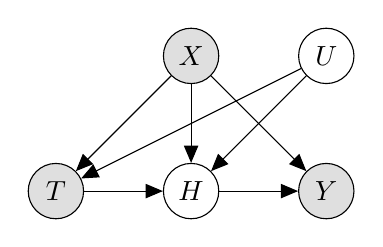
\begin{tikzpicture}

  %
  \node[obs, ]                               (x) {$X$};
  \node[latent, below=of x]                (h) {$H$};
  \node[obs, left=of h]                   (t) {$T$};
  \node[obs, right=of h]                   (y) {$Y$};
  \node[latent, right=of x]                 (u) {$U$};

  %
  \edge {x} {t} ; %
  \edge {x} {h}  ; %
  \edge {x} {y}  ; %
  \edge {t} {h}  ; %
  \edge {h} {y}  ; %
  \edge {u} {t}  ;
  \edge {u} {h}  ;

\end{tikzpicture}}
\caption{\centering \label{fig:confounding:compliance}Response\newline confounding}
\end{subfigure}\quad
\begin{subfigure}{0.22\linewidth}
\centering
\scalebox{0.7}{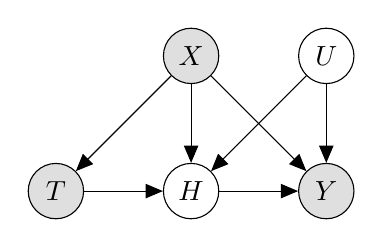
\begin{tikzpicture}

  %
  \node[obs, ]                               (x) {$X$};
  \node[latent, below=of x]                (h) {$H$};
  \node[obs, left=of h]                   (t) {$T$};
  \node[obs, right=of h]                   (y) {$Y$};
  \node[latent, right=of x]                 (u) {$U$};

  %
  \edge {x} {t} ; %
  \edge {x} {h}  ; %
  \edge {x} {y}  ; %
  \edge {t} {h}  ; %
  \edge {h} {y}  ; %
  \edge {u} {h}  ;
  \edge {u} {y}  ;

\end{tikzpicture}}
\caption{\centering \label{fig:confounding:effect}Effect\newline confounding}
\end{subfigure}\quad
\begin{subfigure}{0.22\linewidth}
\centering
\scalebox{0.7}{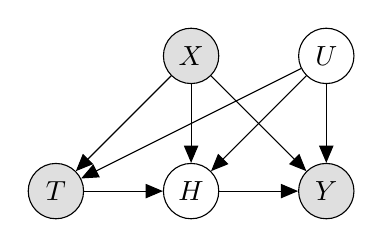
\begin{tikzpicture}

  %
  \node[obs, ]                               (x) {$X$};
  \node[latent, below=of x]                (h) {$H$};
  \node[obs, left=of h]                   (t) {$T$};
  \node[obs, right=of h]                   (y) {$Y$};
  \node[latent, right=of x]                 (u) {$U$};

  %
  \edge {x} {t} ; %
  \edge {x} {h}  ; %
  \edge {x} {y}  ; %
  \edge {t} {h}  ; %
  \edge {h} {y}  ; %
  \edge {u} {t}  ;
  \edge {u} {h}  ;
  \edge {u} {y}  ;

\end{tikzpicture}}
\caption{\centering \label{fig:confounding:total}Total\newline confounding}
\end{subfigure}
\caption{\label{fig:confounding}
The four types of latent confounding in the causal two-groups model.}
\end{figure*}

In this section, we consider how latent confounding impacts statistical inferences in the causal two-groups model. Latent confounding in the C2G model occurs when an unobserved variable $U$ affects two or more of the variables in $\{T, H, Y \}$.  \Cref{fig:confounding} shows the four types of possible latent confounding scenarios.

The key question is whether either of the C2G models proposed above remains \emph{well-specified} under any of these latent confounding scenarios. By well-specified, we mean the observed non-responder and treatment distributions are within the class of probability distributions specified by the modeling assumptions. A well-specified model under latent confounding ensures that integrating out the latent confounder in the untreated group yields the original non-responder distribution and in the treatment group yields the original mixture model,
\begin{equation}
\begin{aligned}
\int p(y | x, u, t=0) p(u) du & = f_0(y \mid x) = p(y | x, h=0, t=1) \, , \\
\int p(y | x, u, t=1) p(u) du &= (1-\pi(x)) f_0(y \mid x) + \pi(x) f_1(y \mid x) \, ,
\end{aligned}
\label{eqn:well-specified}
\end{equation}
where $(\pi, f_0, f_1)$ are specified by the modeling assumptions (i.e. parametric, semi-parametric, or nonparametric). If a model remains well-specified in the presence of latent confounding, statistical inferences will still be valid.

\subsection{Confounding in the additive model}
\label{subsec:confounding:additive}

The additive causal two-groups model requires that the $(f_0, f_1)$ distributions obey \cref{eqn:additive_errors}. Because \cref{eqn:additive_errors} is agnostic to the relationship between $T$ and $H$, it is straightforward to show that the additive causal two groups model remains correctly specified and applicable under response confounding.
\begin{proposition}
\label{prop:compliance-confounding-ac2g}
The additive causal two groups model is robust against response confounding.
\end{proposition}

The story changes when we allow an unobserved random variable to affect the output $Y$. Indeed, even when this variable only affects the conditional means of the non-responder and responder distributions by an additive shift while leaving the noise distribution unchanged, the model is misspecified.

\begin{proposition}
\label{prop:latent-nonrobust-ac2g}
The additive causal two-groups model is misspecified in the presence of an unobserved $U$ such that 
\begin{align*}
Y | X=x, U=u, H=h &=& \mu_{h}(x) + \rho_{h}(u) + \epsilon  \\
\epsilon &\sim& g.
\end{align*}
As a consequence, the additive causal two-groups model is not robust in the presence of canonical, effect, or total confounding.
\end{proposition}


\subsection{Confounding in the nonparametric model}
\label{subsec:confounding:nonparametric}


For the nonparametric method, there are only two modeling assumptions. First, the outcome distribution of the untreated samples must match that of the treated non-responders. Second, the outcome distribution of the treated samples can be written as a mixture model of the form given by \cref{eqn:treatment-mixture}.
The following result shows that this minimalist approach offers an added benefit over the additive model in the form of validity under effect confounding as well as response confounding.

\begin{proposition}
\label{prop:confounding-npc2g}
The nonparametric causal two-groups model is robust against response and effect confounding.
\end{proposition}

The reason why the nonparametric causal two-groups model remains well-specified in the presence of these two types of confounding is that both still allow for $Y \indep T \mid X,  H$. When this conditional independence relationship holds, the non-responder outcome distribution coincides with the untreated outcome distribution. This allows us to write the treatment distribution as the mixture in \cref{eqn:treatment-mixture}, thereby satisfying the conditions of \cref{eqn:well-specified}. When we do not have $Y \indep T \mid X,  H$, we cannot guarantee that the nonparametric causal two-groups model is well-specified, as the following result shows.

\begin{proposition}
\label{prop:canonical-confounding}
The nonparametric causal two-groups model is not robust in the presence of canonical or total confounding.
\end{proposition}

The key to proving \cref{prop:canonical-confounding} is in showing that a canonical confounder $U$ can lead to situations in which the untreated outcome distribution $p(Y \mid X, T=0)$ differs from the treated-but-non-responder outcome distribution $p(Y \mid X, H=0, T=1)$, breaking the fundamental assumptions of the nonparametric causal two-groups model.





%|>>|///////////////////////////////////////////////////////////////////////////////////////////|>>|
%|>>|///////////////////////////////////////////////////////////////////////////////////////////|>>|
%|>>|///////////////////////////////////////////////////////////////////////////////////////////|>>|
% \begin{figure}
% %
% %\begin{subfigure}{0.66\textwidth}
% %
% \includegraphics[width=\textwidth]{errors-and-inconsistent--logistic--nbiht--beta=1.png}
% \caption{\label{fig:error-decay-plot:logistic-regression}
% %This experiment was run under the logistic regression model with \betaXnamelr \(  \betaX = 1  \).
% %The \LHS shows the error decay of BIHT approximations empirically and theoretically.
% %%The empirical results were obtained by running \(  100  \) trials of \(  50  \) iterations of the normalized BIHT algorithm when recovering random \(  k  \)-sparse unit vectors.
% %The \RHS displays the fraction of covariates which fall onto opposite sides of
% %the hyperplanes associated with
% %%the hyperplane whose normal vector is
% %the true parameter, \(  \thetaStar  \), and the approximations.
% %The empirical results were obtained by running \(  100  \) trials of recovering random \(  k  \)-sparse unit vectors via the normalized BIHT algorithm for \(  25  \) iterations.
% %The parameters were set as: \(  d = 2000  \), \(  k = 5  \), \(  n = 3000  \), \(  \epsilonX = 0.25  \), and \(  \rhoX = 0.25  \).%
% This experiment demonstrates the convergence behavior of the normalized BIHT algorithm under logistic regression with \betaXnamelr \(  \betaX = 1  \).
% The left plot shows the empirical and theoretical error decay of the BIHT approximations.
% The right plot shows the fraction of covariates which fall onto opposite sides of
% the hyperplanes associated with
% %the hyperplane whose normal vector is
% the true parameter, \(  \thetaStar  \), and the approximations.
% The experiment ran \(  100  \) trials of recovery for \(  25  \) iterations with parameters: \(  d = 2000  \), \(  k = 5  \), \(  n = 3000  \), \(  \epsilonX = 0.25  \), and \(  \rhoX = 0.25  \).%
% }
% %
% %\Description[Two box plots showing the rates of decay of (1) the error, and (2) the fraction of mismatches in a numerical experiment.]{Two side-by-side box plots displaying the number of iterations of BIHT versus (1) the error, and (2) the fraction of mismatches in a numerical experiment, which are seen to track with the theoretically predicted rates of decay. Results are shown for each of the first 25 iterations.}
% %
% %\end{subfigure}
% \end{figure}
% %|>>|///////////////////////////////////////////////////////////////////////////////////////////|>>|
% %|>>|///////////////////////////////////////////////////////////////////////////////////////////|>>|
% %|>>|///////////////////////////////////////////////////////////////////////////////////////////|>>|

% %|<<|\\\\\\\\\\\\\\\\\\\\\\\\\\\\\\\\\\\\\\\\\\\\\\\\\\\\\\\\\\\\\\\\\\\\\\\\\\\\\\\\\\\\\\\\\\\|<<|
% %|<<|\\\\\\\\\\\\\\\\\\\\\\\\\\\\\\\\\\\\\\\\\\\\\\\\\\\\\\\\\\\\\\\\\\\\\\\\\\\\\\\\\\\\\\\\\\\|<<|
% %|<<|\\\\\\\\\\\\\\\\\\\\\\\\\\\\\\\\\\\\\\\\\\\\\\\\\\\\\\\\\\\\\\\\\\\\\\\\\\\\\\\\\\\\\\\\\\\|<<|
% \begin{figure}
% %\begin{subfigure}{0.33\textwidth}
% %
% \centering
% \includegraphics[width=0.85\textwidth]{m-vs-errors--logistic--nbiht--beta=1.png}
% \caption{\label{fig:m-vs-error-plot:logistic-regression}%
% %This plot shows the (roughly linear) relationship between the number of covariates, \(  d  \), (\(  x  \)-axis) and the reciprocal of the squared error (\(  y  \)-axis), where the error is the \(  \lnorm{2}  \)-distance between the true parameter and the approximation obtained after \(  25  \) iterations of the normalized BIHT algorithm under the logistic regression model with \betaXnamelr \(  \betaX = 1  \).
% %The sparsity and dimension parameters were set, respectively, as: \(  d = 2000  \) and \(  k = 5  \).%
% This experiment studies the relationship between the \errorrate and sample complexity for the normalized BIHT algorithm under logistic regression with \betaXnamelr \(  \betaX = 1  \).
% This plot shows the reciprocal of the squared error (\(  y  \)-axis) scaling roughly linearly with the number of covariates, \(  d  \), (\(  x  \)-axis), where the error is the \(  \lnorm{2}  \)-distance between the true parameter and the approximation obtained after \(  25  \) iterations of the algorithm.
% The experiment ran 100 trials of recovery with dimension and sparsity parameters: \(  d = 2000  \) and \(  k = 5  \).%
% }
% %
% %\Description[A box plot of the relationship between the number of measurements and reciprocal of the error in a numerical experiment.]{A box plot displaying the approximately linear scaling of the number of measurements versus the reciprocal of the error in a numerical experiment, where the number of measurements is varied between 100 and 2000 at increments of 100.}
% %\end{subfigure}
% \end{figure}
% %|<<|\\\\\\\\\\\\\\\\\\\\\\\\\\\\\\\\\\\\\\\\\\\\\\\\\\\\\\\\\\\\\\\\\\\\\\\\\\\\\\\\\\\\\\\\\\\|<<|
% %|<<|\\\\\\\\\\\\\\\\\\\\\\\\\\\\\\\\\\\\\\\\\\\\\\\\\\\\\\\\\\\\\\\\\\\\\\\\\\\\\\\\\\\\\\\\\\\|<<|
% %|<<|\\\\\\\\\\\\\\\\\\\\\\\\\\\\\\\\\\\\\\\\\\\\\\\\\\\\\\\\\\\\\\\\\\\\\\\\\\\\\\\\\\\\\\\\\\\|<<|

% %|>>|///////////////////////////////////////////////////////////////////////////////////////////|>>|
% %|>>|///////////////////////////////////////////////////////////////////////////////////////////|>>|
% %|>>|///////////////////////////////////////////////////////////////////////////////////////////|>>|
% \begin{figure}
% %
% %\begin{subfigure}{0.66\textwidth}
% %
% \includegraphics[width=\textwidth]{errors-and-inconsistent--probit--nbiht--beta=1.png}
% \caption{\label{fig:error-decay-plot:probit}
% %This experiment was run under the probit regression model with \betaXnamepr \(  \betaX = 1  \).
% %The \LHS shows the empirical and theoretical error decay of the BIHT approximations.
% %The \RHS shows the fraction of covariates which fall onto opposite sides of
% %the hyperplanes associated with
% %%the hyperplane whose normal vector is
% %the true parameter, \(  \thetaStar  \), and the approximations.
% %The experiment ran \(  100  \) trials of recovery with the normalized BIHT algorithm for \(  25  \) iterations under the probit regression model with \betaXnamepr \(  \betaX = 1  \) with the parameters: \(  d = 2000  \), \(  k = 5  \), \(  n = 3000  \), \(  \epsilonX = 0.25  \), and \(  \rhoX = 0.25  \).%
% This experiment demonstrates the convergence behavior of the normalized BIHT algorithm under probit regression with \betaXnamepr \(  \betaX = 1  \).
% The left plot shows the empirical and theoretical error decay of the BIHT approximations.
% The right plot shows the fraction of covariates which fall onto opposite sides of
% the hyperplanes associated with
% %the hyperplane whose normal vector is
% the true parameter, \(  \thetaStar  \), and the approximations.
% The experiment ran \(  100  \) trials of recovery for \(  25  \) iterations with parameters: \(  d = 2000  \), \(  k = 5  \), \(  n = 3000  \), \(  \epsilonX = 0.25  \), and \(  \rhoX = 0.25  \).%
% }
% %
% %\Description[Two box plots showing the rates of decay of (1) the error, and (2) the fraction of mismatches in a numerical experiment.]{Two side-by-side box plots displaying the number of iterations of BIHT versus (1) the error, and (2) the fraction of mismatches in a numerical experiment, which are seen to track with the theoretically predicted rates of decay. Results are shown for each of the first 25 iterations.}
% %
% %\end{subfigure}
% \end{figure}
% %|>>|///////////////////////////////////////////////////////////////////////////////////////////|>>|
% %|>>|///////////////////////////////////////////////////////////////////////////////////////////|>>|
% %|>>|///////////////////////////////////////////////////////////////////////////////////////////|>>|

% %|<<|\\\\\\\\\\\\\\\\\\\\\\\\\\\\\\\\\\\\\\\\\\\\\\\\\\\\\\\\\\\\\\\\\\\\\\\\\\\\\\\\\\\\\\\\\\\|<<|
% %|<<|\\\\\\\\\\\\\\\\\\\\\\\\\\\\\\\\\\\\\\\\\\\\\\\\\\\\\\\\\\\\\\\\\\\\\\\\\\\\\\\\\\\\\\\\\\\|<<|
% %|<<|\\\\\\\\\\\\\\\\\\\\\\\\\\\\\\\\\\\\\\\\\\\\\\\\\\\\\\\\\\\\\\\\\\\\\\\\\\\\\\\\\\\\\\\\\\\|<<|
% \begin{figure}
% %\begin{subfigure}{0.33\textwidth}
% %
% \centering
% \includegraphics[width=0.85\textwidth]{m-vs-errors--probit--nbiht--beta=1.png}
% \caption{\label{fig:m-vs-error-plot:probit}%
% %This plot shows the (roughly linear) relationship between the number of covariates, \(  d  \), (\(  x  \)-axis) and the reciprocal of the squared error (\(  y  \)-axis), where the error is the \(  \lnorm{2}  \)-distance between the true parameter and the approximation obtained after \(  25  \) iterations of the normalized BIHT algorithm under the probit regression model with \betaXnamepr \(  \betaX = 1  \).
% %The sparsity and dimension parameters were set, respectively, as: \(  d = 2000  \) and \(  k = 5  \).%
% This experiment studies the relationship between the \errorrate and sample complexity for the normalized BIHT algorithm under probit regression with \betaXnamepr \(  \betaX = 1  \).
% This plot shows the reciprocal of the squared error (\(  y  \)-axis) scaling roughly linearly with the number of covariates, \(  d  \), (\(  x  \)-axis), where the error is the \(  \lnorm{2}  \)-distance between the true parameter and the approximation obtained after \(  25  \) iterations of the algorithm.
% The experiment ran 100 trials of recovery with dimension and sparsity parameters: \(  d = 2000  \) and \(  k = 5  \).%
% }
% %
% %\Description[A box plot of the relationship between the number of measurements and reciprocal of the error in a numerical experiment.]{A box plot displaying the approximately linear scaling of the number of measurements versus the reciprocal of the error in a numerical experiment, where the number of measurements is varied between 100 and 2000 at increments of 100.}
% %\end{subfigure}
% \end{figure}
% %|<<|\\\\\\\\\\\\\\\\\\\\\\\\\\\\\\\\\\\\\\\\\\\\\\\\\\\\\\\\\\\\\\\\\\\\\\\\\\\\\\\\\\\\\\\\\\\|<<|
% %|<<|\\\\\\\\\\\\\\\\\\\\\\\\\\\\\\\\\\\\\\\\\\\\\\\\\\\\\\\\\\\\\\\\\\\\\\\\\\\\\\\\\\\\\\\\\\\|<<|
% %|<<|\\\\\\\\\\\\\\\\\\\\\\\\\\\\\\\\\\\\\\\\\\\\\\\\\\\\\\\\\\\\\\\\\\\\\\\\\\\\\\\\\\\\\\\\\\\|<<|

% %|>>|///////////////////////////////////////////////////////////////////////////////////////////|>>|
% %|>>|///////////////////////////////////////////////////////////////////////////////////////////|>>|
% %|>>|///////////////////////////////////////////////////////////////////////////////////////////|>>|
\begin{figure}
%
%\begin{subfigure}{0.66\textwidth}
%
\includegraphics[width=\textwidth]{errors--logistic--nbiht-beta=1.png}
\includegraphics[width=\textwidth]{errors--logistic--biht-beta=1.png}
\caption{\label{fig:error-decay-nbiht-biht-comparison-beta=1-plot:logistic-regression}
This experiment compares the iterative approximation errors for BIHT with (top plot) and without (bottom plot) the normalization step of the algorithm under logistic regression with \betaXnamelr \(  \betaX = 1  \).
The error is the \(  \lnorm{2}  \)-distance between the normalized approximation and the true parameter.
In both plots, the theoretical error decay for the normalized version of BIHT with logistic regression is displayed for reference.
The experiment ran \(  100  \) trials of recovery for \(  30  \) iterations with parameters: \(  d = 2000  \), \(  k = 5  \), \(  n = 3000  \), \(  \epsilonX = 0.25  \), and \(  \rhoX = 0.25  \).%
}
%
%\end{subfigure}
\end{figure}
%|>>|///////////////////////////////////////////////////////////////////////////////////////////|>>|
%|>>|///////////////////////////////////////////////////////////////////////////////////////////|>>|
%|>>|///////////////////////////////////////////////////////////////////////////////////////////|>>|

%|>>|///////////////////////////////////////////////////////////////////////////////////////////|>>|
%|>>|///////////////////////////////////////////////////////////////////////////////////////////|>>|
%|>>|///////////////////////////////////////////////////////////////////////////////////////////|>>|
\begin{figure}
%
%\begin{subfigure}{0.66\textwidth}
%
\includegraphics[width=\textwidth]{errors--sign--nbiht.png}
\includegraphics[width=\textwidth]{errors--sign--biht.png}
\caption{\label{fig:error-decay-nbiht-biht-comparison-beta=1-plot:sign}
This experiment compares the iterative approximation errors for BIHT with (top plot) and without (bottom plot) the normalization step of the algorithm under the noiseless model.
The error is the \(  \lnorm{2}  \)-distance between the normalized approximation and the true parameter.
In both plots, the theoretical error decay for the normalized version of BIHT in the noiseless setting---established by \cite{matsumoto2022binary}---is displayed for reference.
The experiment ran \(  100  \) trials of recovery for \(  30  \) iterations with parameters: \(  d = 2000  \), \(  k = 5  \), \(  n = 700  \), \(  \epsilonX = 0.25  \), and \(  \rhoX = 0.25  \).%
}
%
%\end{subfigure}
\end{figure}
%|>>|///////////////////////////////////////////////////////////////////////////////////////////|>>|
%|>>|///////////////////////////////////////////////////////////////////////////////////////////|>>|
%|>>|///////////////////////////////////////////////////////////////////////////////////////////|>>|

\begin{comment}

%|>>|///////////////////////////////////////////////////////////////////////////////////////////|>>|
%|>>|///////////////////////////////////////////////////////////////////////////////////////////|>>|
%|>>|///////////////////////////////////////////////////////////////////////////////////////////|>>|
\begin{figure}
%
%\begin{subfigure}{0.66\textwidth}
%
\includegraphics[width=\textwidth]{lr-nbiht-errors-and-inconsistent-n=2000-k=5-m=1000-epsilon=0.05-rho=0.05-num_trials=100-figsize=(28, 6)--2-1--cropped.png}%{lr-nbiht-errors-and-inconsistent-n=2000-k=5-m=1000-epsilon=0.05-rho=0.05-num_trials=100--2-1b.png}
\caption{\label{fig:error-decay-plot:logistic-regression}
This experiment was run under the logistic regression model with \betaXnamelr \(  \betaX = 1  \).
The \LHS shows the error decay of BIHT approximations empirically and theoretically.
%The empirical results were obtained by running \(  100  \) trials of \(  50  \) iterations of the normalized BIHT algorithm when recovering random \(  k  \)-sparse unit vectors.
The \RHS displays the fraction of covariates which fall onto opposite sides of
the hyperplanes associated with
%the hyperplane whose normal vector is
the true parameter, \(  \thetaStar  \), and the approximations.
The empirical results were obtained by running \(  100  \) trials of recovering random \(  k  \)-sparse unit vectors via the normalized BIHT algorithm for \(  25  \) iterations.
The parameters were set as: \(  d = 2000  \), \(  k = 5  \), \(  n = 1000  \), \(  \epsilonX = 0.05  \), and \(  \rhoX = 0.05  \).%
}
%
%\Description[Two box plots showing the rates of decay of (1) the error, and (2) the fraction of mismatches in a numerical experiment.]{Two side-by-side box plots displaying the number of iterations of BIHT versus (1) the error, and (2) the fraction of mismatches in a numerical experiment, which are seen to track with the theoretically predicted rates of decay. Results are shown for each of the first 25 iterations.}
%
%\end{subfigure}
\end{figure}
%|>>|///////////////////////////////////////////////////////////////////////////////////////////|>>|
%|>>|///////////////////////////////////////////////////////////////////////////////////////////|>>|
%|>>|///////////////////////////////////////////////////////////////////////////////////////////|>>|

%|<<|\\\\\\\\\\\\\\\\\\\\\\\\\\\\\\\\\\\\\\\\\\\\\\\\\\\\\\\\\\\\\\\\\\\\\\\\\\\\\\\\\\\\\\\\\\\|<<|
%|<<|\\\\\\\\\\\\\\\\\\\\\\\\\\\\\\\\\\\\\\\\\\\\\\\\\\\\\\\\\\\\\\\\\\\\\\\\\\\\\\\\\\\\\\\\\\\|<<|
%|<<|\\\\\\\\\\\\\\\\\\\\\\\\\\\\\\\\\\\\\\\\\\\\\\\\\\\\\\\\\\\\\\\\\\\\\\\\\\\\\\\\\\\\\\\\\\\|<<|
\begin{figure}
%\begin{subfigure}{0.33\textwidth}
%
\centering
\includegraphics[width=0.85\textwidth]{lr-nbiht-m-vs-errors--n=2000-k=5-m=[100-2000]-epsilon=0.1-rho=0.05-num_trials=100-figsize=(24, 6)--2-1--cropped.png}%{lr-nbiht-m-vs-errors--n=2000-k=5-m=[100-2000]-epsilon=0.1-rho=0.05-num_trials=100--2-1b.png}
\caption{\label{fig:m-vs-error-plot:logistic-regression}%
This plot shows the (roughly linear) relationship between the number of covariates, \(  d  \), (\(  x  \)-axis) and the reciprocal of the squared error (\(  y  \)-axis), where the error is the \(  \lnorm{2}  \)-distance between the true parameter and the approximation obtained after \(  25  \) iterations of the normalized BIHT algorithm under the logistic regression model with \betaXnamelr \(  \betaX = 1  \).
The sparsity and dimension parameters were set, respectively, as: \(  d = 2000  \) and \(  k = 5  \).%
}
%
%\Description[A box plot of the relationship between the number of measurements and reciprocal of the error in a numerical experiment.]{A box plot displaying the approximately linear scaling of the number of measurements versus the reciprocal of the error in a numerical experiment, where the number of measurements is varied between 100 and 2000 at increments of 100.}
%\end{subfigure}
\end{figure}
%|<<|\\\\\\\\\\\\\\\\\\\\\\\\\\\\\\\\\\\\\\\\\\\\\\\\\\\\\\\\\\\\\\\\\\\\\\\\\\\\\\\\\\\\\\\\\\\|<<|
%|<<|\\\\\\\\\\\\\\\\\\\\\\\\\\\\\\\\\\\\\\\\\\\\\\\\\\\\\\\\\\\\\\\\\\\\\\\\\\\\\\\\\\\\\\\\\\\|<<|
%|<<|\\\\\\\\\\\\\\\\\\\\\\\\\\\\\\\\\\\\\\\\\\\\\\\\\\\\\\\\\\\\\\\\\\\\\\\\\\\\\\\\\\\\\\\\\\\|<<|

%|>>|///////////////////////////////////////////////////////////////////////////////////////////|>>|
%|>>|///////////////////////////////////////////////////////////////////////////////////////////|>>|
%|>>|///////////////////////////////////////////////////////////////////////////////////////////|>>|
\begin{figure}
%
%\begin{subfigure}{0.66\textwidth}
%
\includegraphics[width=\textwidth]{pr-nbiht-errors-and-inconsistent-n=2000-k=5-m=1000-epsilon=0.05-rho=0.05-num_trials=100-figsize=(28, 6)--2-1--cropped.png}%{pr-nbiht-errors-and-inconsistent-n=2000-k=5-m=1000-epsilon=0.05-rho=0.05-num_trials=100--2-1c.png}
\caption{\label{fig:error-decay-plot:probit}
This experiment was run under the probit regression model with \betaXnamepr \(  \betaX = 1  \).
The \LHS shows the error decay of BIHT approximations empirically and theoretically.
%The empirical results were obtained by running \(  100  \) trials of \(  50  \) iterations of the normalized BIHT algorithm when recovering random \(  k  \)-sparse unit vectors.
The \RHS displays the fraction of covariates which fall onto opposite sides of
the hyperplanes associated with
%the hyperplane whose normal vector is
the true parameter, \(  \thetaStar  \), and the approximations.
The empirical results were obtained by running \(  100  \) trials of recovering random \(  k  \)-sparse unit vectors via the normalized BIHT algorithm for \(  25  \) iterations.
The parameters were set as: \(  d = 2000  \), \(  k = 5  \), \(  n = 1000  \), \(  \epsilonX = 0.05  \), and \(  \rhoX = 0.05  \).%
}
%
%\Description[Two box plots showing the rates of decay of (1) the error, and (2) the fraction of mismatches in a numerical experiment.]{Two side-by-side box plots displaying the number of iterations of BIHT versus (1) the error, and (2) the fraction of mismatches in a numerical experiment, which are seen to track with the theoretically predicted rates of decay. Results are shown for each of the first 25 iterations.}
%
%\end{subfigure}
\end{figure}
%|>>|///////////////////////////////////////////////////////////////////////////////////////////|>>|
%|>>|///////////////////////////////////////////////////////////////////////////////////////////|>>|
%|>>|///////////////////////////////////////////////////////////////////////////////////////////|>>|

%|<<|\\\\\\\\\\\\\\\\\\\\\\\\\\\\\\\\\\\\\\\\\\\\\\\\\\\\\\\\\\\\\\\\\\\\\\\\\\\\\\\\\\\\\\\\\\\|<<|
%|<<|\\\\\\\\\\\\\\\\\\\\\\\\\\\\\\\\\\\\\\\\\\\\\\\\\\\\\\\\\\\\\\\\\\\\\\\\\\\\\\\\\\\\\\\\\\\|<<|
%|<<|\\\\\\\\\\\\\\\\\\\\\\\\\\\\\\\\\\\\\\\\\\\\\\\\\\\\\\\\\\\\\\\\\\\\\\\\\\\\\\\\\\\\\\\\\\\|<<|
\begin{figure}
%\begin{subfigure}{0.33\textwidth}
%
\centering
\includegraphics[width=0.85\textwidth]{pr-nbiht-m-vs-errors--n=2000-k=5-m=[100-2000]-epsilon=0.1-rho=0.05-num_trials=100-figsize=(24, 6)--2-1--cropped.png}%{pr-nbiht-m-vs-errors--n=2000-k=5-m=[100-2000]-epsilon=0.1-rho=0.05-num_trials=100--2-1f.png}
\caption{\label{fig:m-vs-error-plot:probit}%
This plot shows the (roughly linear) relationship between the number of covariates, \(  d  \), (\(  x  \)-axis) and the reciprocal of the squared error (\(  y  \)-axis), where the error is the \(  \lnorm{2}  \)-distance between the true parameter and the approximation obtained after \(  25  \) iterations of the normalized BIHT algorithm under the probit regression model with \betaXnamepr \(  \betaX = 1  \).
The sparsity and dimension parameters were set, respectively, as: \(  d = 2000  \) and \(  k = 5  \).%
}
%
%\Description[A box plot of the relationship between the number of measurements and reciprocal of the error in a numerical experiment.]{A box plot displaying the approximately linear scaling of the number of measurements versus the reciprocal of the error in a numerical experiment, where the number of measurements is varied between 100 and 2000 at increments of 100.}
%\end{subfigure}
\end{figure}
%|<<|\\\\\\\\\\\\\\\\\\\\\\\\\\\\\\\\\\\\\\\\\\\\\\\\\\\\\\\\\\\\\\\\\\\\\\\\\\\\\\\\\\\\\\\\\\\|<<|
%|<<|\\\\\\\\\\\\\\\\\\\\\\\\\\\\\\\\\\\\\\\\\\\\\\\\\\\\\\\\\\\\\\\\\\\\\\\\\\\\\\\\\\\\\\\\\\\|<<|
%|<<|\\\\\\\\\\\\\\\\\\\\\\\\\\\\\\\\\\\\\\\\\\\\\\\\\\\\\\\\\\\\\\\\\\\\\\\\\\\\\\\\\\\\\\\\\\\|<<|

\end{comment}

\begin{figure}[htb]
\small
\begin{tcolorbox}[left=3pt,right=3pt,top=3pt,bottom=3pt,title=\textbf{Conversation History:}]
[human]: Craft an intriguing opening paragraph for a fictional short story. The story should involve a character who wakes up one morning to find that they can time travel.

...(Human-Bot Dialogue Turns)... \textcolor{blue}{(Topic: Time-Travel Fiction)}

[human]: Please describe the concept of machine learning. Could you elaborate on the differences between supervised, unsupervised, and reinforcement learning? Provide real-world examples of each.

...(Human-Bot Dialogue Turns)... \textcolor{blue}{(Topic: Machine learning Concepts and Types)}


[human]: Discuss antitrust laws and their impact on market competition. Compare the antitrust laws in US and China along with some case studies

...(Human-Bot Dialogue Turns)... \textcolor{blue}{(Topic: Antitrust Laws and Market Competition)}

[human]: The vertices of a triangle are at points (0, 0), (-1, 1), and (3, 3). What is the area of the triangle?

...(Human-Bot Dialogue Turns)... \textcolor{blue}{(Topic: Area and Circumcircle of Triangle)}

...(Human-Bot Dialogue Interaction on Other Topics)... 

\end{tcolorbox}
\begin{tcolorbox}[left=3pt,right=3pt,top=3pt,bottom=3pt,title=\textbf{Question:}]
What title reflects the thematic essence of the Doctor's experience with time travel as described in the story?
\end{tcolorbox}
\begin{tcolorbox}[left=3pt,right=3pt,top=3pt,bottom=3pt,title=\textbf{Ground-Truth Answer:}]
Awakening to Eternity: The Doctor's New Dawn
\end{tcolorbox}
\begin{tcolorbox}[left=3pt,right=3pt,top=3pt,bottom=3pt,title=\textbf{Retrieved Memory (Turn-Level):}]
[human]: Describe the process and write out the balanced chemical equation for the reaction that occurs when solid calcium carbonate reacts with hydrochloric acid to form aqueous calcium chloride, carbon dioxide, and water. What type of reaction is this, and what observations might indicate that the reaction is taking place?

[bot]: When solid calcium carbonate ($\text{CaCO}_{3}$) reacts with hydrochloric acid (HCl), the products formed are aqueous calcium chloride ($\text{CaCl}_{2}$), carbon dioxide ($\text{CO}_{2}$), and water ($\text{H}_{2}\text{O}$). The balanced chemical equation for this reaction is: ... \textcolor{blue}{(Topic: Calcium Carbonate and Hydrochloric Acid Reaction)}

\textcolor{brown}{
[human]: Write a title for your story.}

\textcolor{brown}{
[bot]: "Awakening to Eternity: The Doctor's New Dawn".
} \textcolor{blue}{(Topic: Time-Travel Fiction)}

[human]: Analyze the following customer reviews from different sources for three different smartphones - the latest iPhone, Samsung Galaxy, and Google Pixel - and provide an overall rating for each phone on a scale of 1 to 10. Consider the following complex and contradictory reviews: - TechRadar's review of the latest iPhone: The new iPhone is a stunning triumph of engineering that sets a new bar for smartphone performance and camera quality. However, the incremental design and high price mean it lacks the 'wow' factor of previous iPhones. Still, its power and intelligence are unrivaled. - CNET's review of the latest Samsung Galaxy: ... Return the answer as a JSON object with the overall ratings for each phone out of 10, to one decimal place.

[bot]: ```json { "iPhone": 8.5, "Samsung Galaxy": 8.0, "Google Pixel": 7.5 } ```

\textcolor{blue}{(Topic: Smartphone Review Ratings Analysis)}
\end{tcolorbox}
\begin{tcolorbox}[left=3pt,right=3pt,top=3pt,bottom=3pt,title=\textbf{Answer (Turn-Level Retrieval):}]
As an AI language model, I do not have access to the story you mentioned earlier. Please provide me with the story or the necessary details so that I can assist you better.

\textbf{\textcolor{red}{(The next part of this figure~\ref{fig: case_study_segment_vs_turn} will be continued on the next page.)}}
\end{tcolorbox}
\end{figure}

\begin{figure}[htb]
% \ContinuedFloat
\small
\begin{tcolorbox}[left=3pt,right=3pt,top=3pt,bottom=3pt,title=\textbf{Retrieved Memory (Ours):}]
[human]: Craft an intriguing opening paragraph for a fictional short story. The story should involve a character who wakes up one morning to find that they can time travel.

[bot]: In the hushed pre-dawn hours, when the world still slumbers under the cloak of night, Alex found themselves caught in the fragile boundary between sleep and wakefulness. ...

[human]: Summarize the story with three bullet points using only nouns and adjectives, without verbs.

[bot]: - Alex, pre-dawn awakening, time-travel discovery - Disorientation, vertigo, reality's malleability - Sunlight, new day, astonishing truth

[human]: Is there any famous fictional character that can time travel? If so, can you rewrite your story with him or her?

[bot]: - \textcolor{brown}{Doctor Who, a renowned time-traveling character from British television, is a perfect fit for this scenario.} In the silent embrace of early morning, where shadows merge with the fading night, the Doctor found themselves in the thin veil separating dreams from consciousness. It was here, amidst the soft whispers of time, that an unusual sensation enveloped them—a sense of time's fabric slipping through their fingers like grains of sand. As dawn's light broke through the darkness, painting the room in hues of gold and amber, the Doctor's eyes opened to what appeared to be an ordinary day. \textcolor{brown}{However, upon standing, a wave of dizziness overwhelmed them, the surroundings blurred, and in that moment of confusion, the Doctor realized a profound truth: they had not only awakened to a new dawn but had also stumbled upon the incredible ability to navigate the currents of time at will.}

\textcolor{brown}{[human]: Write a title for your story.}

\textcolor{brown}{[bot]: "Awakening to Eternity: The Doctor's New Dawn"} \textcolor{blue}{(Topic: Time-Travel Fiction)}
\end{tcolorbox}
\begin{tcolorbox}[left=3pt,right=3pt,top=3pt,bottom=3pt,title=\textbf{Answer (Ours):}]
The title "Awakening to Eternity: The Doctor's New Dawn" reflects the thematic essence of the Doctor's experience with time travel as described in the story. It captures the idea of a new beginning, a sense of eternity, and the awakening of a new power that will change the course of the Doctor's life forever.
\end{tcolorbox}
\caption{Case study comparing our \sysname\ with the \textit{turn-level} memory baseline. When constructing the memory bank at the \textit{turn-level}, the agent fails to provide a satisfactory response due to fragmentation: the retrieved dialogue turns can not capture a complete human-agent interaction related to the query, missing critical information highlighted in \textcolor{brown}{brown}. The dialogue topic is emphasized in \textcolor{blue}{blue}. Some context is omitted (replaced by ...) due to length constraints.}
\label{fig: case_study_segment_vs_turn}
\end{figure}

\newpage

\begin{figure}[htbp]
\small
\begin{tcolorbox}[left=3pt,right=3pt,top=3pt,bottom=3pt,title=\textbf{Conversation History:}]
[human]: Explain what's base rate fallacy and list five specific examples of ...

... (Human-Bot Dialogue Turns) ... \textcolor{blue}{(Topic: Base Rate Fallacy In Politics)}


[human]: How many integers are in the solution of the inequality $|x + 5| < 10$?

... (Human-Bot Dialogue Turns) ... \textcolor{blue}{(Topic: Number of Integers in Inequalities)}

[human]: How have the Alps and Rhine River influenced settlement and agriculture in Western Europe?

... (Human-Bot Dialogue Turns) ... \textcolor{blue}{(Topic: Alps and Rhine River Impact)}

[human]: In a survey conducted at a local high school, preferences for a new school color were measured: 58\% of students liked the color blue, 45\% preferred green, and 22\% liked both colors. If we randomly pick a student from the school, what's the probability that they would like neither blue nor green?

... (Human-Bot Dialogue Turns) ... \textcolor{blue}{(Topic: Probability of Liking Colors in Survey)}

[human]: Imagine you are participating in a race with a group of people. If you have just overtaken the second person, what's your current position? Where is the person you just overtook?

... (Human-Bot Dialogue Turns) ... \textcolor{blue}{(Topic: Overtaking Positions in Race)}
\end{tcolorbox}
\begin{tcolorbox}[left=3pt,right=3pt,top=3pt,bottom=3pt,title=\textbf{Question:}]
[human]: In the inequality question, how many positive integers are in the solution of the second inequality?
\end{tcolorbox}
\begin{tcolorbox}[left=3pt,right=3pt,top=3pt,bottom=3pt,title=\textbf{Ground-Truth Answer:}]
In the second inequality, $(|x + 10| < 5)$, the solution range is $(-15 < x < -5)$. Within this range, there are no positive integers, as all values of $(x)$ that satisfy the inequality are negative.
\end{tcolorbox}
\begin{tcolorbox}[left=3pt,right=3pt,top=3pt,bottom=3pt,title=\textbf{Retrieved Memory (Session-Level):}]
[human]: Explain what's base rate fallacy and list five specific examples of ...

... (Human-Bot Dialogue Turns) ... \textcolor{blue}{(Topic: Base Rate Fallacy In Politics)}

[human]: How many integers are in the solution of the inequality $|x + 5| < 10$?

[bot]: To solve the inequality $|x + 5| < 10$, ... 

\textcolor{brown}{
[human]: What about $|x + 10| < 5$?
}

\textcolor{brown}{
[bot]: To solve the inequality $|x + 10| < 5$, we ...} \textcolor{gray}{(``overwhelmed'' by other irrelevant, redundant content)}

... (Human-Bot Dialogue Turns) ...  \textcolor{blue}{(Topic: Number of Integers in Inequalities)}

% \textcolor{brown}{
% [human]: What about $|x + 10| < 5$
% }

% \textcolor{brown}{
% [bot]: To solve the inequality $|x + 10| < 5$, ...
% } \textcolor{blue}{(Topic: Number of Integers in Inequalities)}

[human]: How have the Alps and Rhine River influenced settlement and agriculture in Western Europe?

... (Human-Bot Dialogue Turns) ... \textcolor{blue}{(Topic: Alps and Rhine River Impact)}

[human]: In a survey conducted at a local high school, ...

... (Human-Bot Dialogue Turns) ... \textcolor{blue}{(Topic: Probability of Liking Colors in Survey)}
\end{tcolorbox}
\begin{tcolorbox}[left=3pt,right=3pt,top=3pt,bottom=3pt,title=\textbf{Answer (Session-Level Retrieval):}]
I apologize for the confusion earlier. To answer your question, the second inequality was not provided in our previous conversation. If you could provide the inequality, I would be happy to help you find the solution and the number of positive integers in the solution set.

\textbf{\textcolor{red}{(The next part of this figure~\ref{fig: case_study_segment_vs_session} will be continued on the next page.)}}
\end{tcolorbox}
\end{figure}
\begin{figure}[htbp]
% \ContinuedFloat
\small
\begin{tcolorbox}[left=3pt,right=3pt,top=3pt,bottom=3pt,title=\textbf{Retrieved Memory (Ours):}]
[human]: How many integers are in the solution of the inequality $|x + 5| < 10$?

[bot]: To solve the inequality $|x + 5| < 10$, we break it into two cases based on the definition of absolute value: 
1. $x + 5 < 10$ 
2. $-(x + 5) < 10$, which simplifies to $x + 5 > -10$ 
Solving each case: 
1. $x < 5$ 
2. $x > -15$ 
Combining these, we get $-15 < x < 5$. This inequality means that $x$ can be any number greater than $-15$ and less than $5$. To find how many integers satisfy this condition, we list them: $-14, -13, -12, -11, -10, -9, -8, -7, -6, -5, -4, -3, -2, -1, 0, 1, 2, 3, 4$. There are 19 integers that satisfy the inequality $|x + 5| < 10$.

\textcolor{brown}{
[human]: What about $|x + 10| < 5$?
}

\textcolor{brown}{
[bot]: To solve the inequality $|x + 10| < 5$, we again consider two cases: 
1. $x + 10 < 5$ 
2. $-(x + 10) < 5$, which simplifies to $x + 10 > -5$ 
Solving each case: 
1. $x < -5$ 
2. $x > -15$ 
Combining these, we get $-15 < x < -5$. This inequality means that $x$ can be any number greater than $-15$ and less than $-5$. To find how many integers satisfy this condition, we list them: $-14, -13, -12, -11, -10, -9, -8, -7, -6$. There are 9 integers that satisfy the inequality $|x + 10| < 5$.
}

[human]: What about $|x + 10| < 10$?

[bot]: To solve the inequality $|x + 10| < 10$, we consider two cases: 
1. $x + 10 < 10$ 
2. $-(x + 10) < 10$, which simplifies to $x + 10 > -10$ 
Solving each case: 
1. $x < 0$ 
2. $x > -20$ 
Combining these, we get $-20 < x < 0$. This inequality means that $x$ can be any number greater than $-20$ and less than $0$. To find how many integers satisfy this condition, we list them: $-19, -18, -17, -16, -15, -14, -13, -12, -11, -10, -9, -8, -7, -6, -5, -4, -3, -2, -1$. There are 19 integers that satisfy the inequality $|x + 10| < 10$. \textcolor{blue}{(Topic: Number of Integers in Inequalities)}
\end{tcolorbox}
\begin{tcolorbox}[left=3pt,right=3pt,top=3pt,bottom=3pt,title=\textbf{Answer (Ours):}]
To find the number of positive integers that satisfy the inequality $(|x + 10| < 5)$, we need to look for positive integers in the solution set $(-15 < x < -5)$. Since there are no positive integers in this interval, the answer is 0.

\end{tcolorbox}
\caption{Case study comparing our \sysname\ with the \textit{session-level} memory baseline. When constructing the memory bank at the \textit{session-level}, the agent fails to provide a satisfactory response due to the inclusion of excessive irrelevant information within a session. This distracts the generator from focusing on the truly useful information highlighted in \textcolor{brown}{brown}. The dialogue topic is emphasized in \textcolor{blue}{blue}. Some context is omitted (replaced by ...) due to length constraints.}
\label{fig: case_study_segment_vs_session}
\end{figure}



\begin{figure}[htb]
\small
\begin{tcolorbox}[left=3pt,right=3pt,top=3pt,bottom=3pt,title=\textbf{Conversation History:}]
[human]: Photosynthesis is a vital process for life on Earth. Could you outline the two main stages of photosynthesis, including where they take place within the chloroplast, and the primary inputs and outputs for each stage? ... (Human-Bot Dialogue Turns)... \textcolor{blue}{(Topic: Photosynthetic Energy Production)}

[human]: Please assume the role of an English translator, tasked with correcting and enhancing spelling and language. Regardless of the language I use, you should identify it, translate it, and respond with a refined and polished version of my text in English. 

... (Human-Bot Dialogue Turns)...  \textcolor{blue}{(Topic: Language Translation and Enhancement)}

[human]: Suggest five award-winning documentary films with brief background descriptions for aspiring filmmakers to study.

\textcolor{brown}{[bot]: ...
5. \"An Inconvenient Truth\" (2006) - Directed by Davis Guggenheim and featuring former United States Vice President Al Gore, this documentary aims to educate the public about global warming. It won two Academy Awards, including Best Documentary Feature. The film is notable for its straightforward yet impactful presentation of scientific data, making complex information accessible and engaging, a valuable lesson for filmmakers looking to tackle environmental or scientific subjects.}

... (Human-Bot Dialogue Turns)... 
\textcolor{blue}{(Topic: Documentary Films Recommendation)}

[human]: Given the following records of stock prices, extract the highest and lowest closing prices for each month in the year 2022. Return the results as a CSV string, with one line allocated for each month. Date,Open,High,Low,Close,Volume ... ... (Human-Bot Dialogue Turns)...  \textcolor{blue}{(Topic: Stock Prices Analysis)}

[human]: The city of Vega intends to build a bridge that will span the Vegona River, covering a distance of 1.8 kilometers. The proposed location falls within a seismically active area that has experienced several high-magnitude earthquakes. Given these circumstances, what would be the best approach to constructing the bridge? ... (Human-Bot Dialogue Turns)...  \textcolor{blue}{(Topic: Seismic Bridge Construction)}
\end{tcolorbox}
\begin{tcolorbox}[left=3pt,right=3pt,top=3pt,bottom=3pt,title=\textbf{Question:}]
Which documentary won two Academy Awards and what lesson does it offer to filmmakers?
\end{tcolorbox}
\begin{tcolorbox}[left=3pt,right=3pt,top=3pt,bottom=3pt,title=\textbf{Ground-Truth Answer:}]
``An Inconvenient Truth" (2006) won two Academy Awards. It offers the lesson of making complex information accessible and engaging, a valuable lesson for filmmakers looking to tackle environmental or scientific subjects.
\end{tcolorbox}
\begin{tcolorbox}[left=3pt,right=3pt,top=3pt,bottom=3pt,title=\textbf{Memory generated by RecurSum~\citep{wang2023recursively}:}]
The dialogue provided detailed information on various topics, including the stages of photosynthesis, energy production estimates through photosynthesis for different organisms, translations and enhancements of phrases in different languages, recommendations for documentary films, a pitch for a film about overcoming adversity, analysis of stock prices, and considerations for constructing a bridge in a seismically active area. Here's a summary of the key points: ...

\textbf{Documentary Film Recommendations}: Suggested five award-winning documentary films for aspiring filmmakers to study, with brief background descriptions for each. The response included:

-  "March of the Penguins" (2005) - Emperor penguins' journey in Antarctica; noted for its cinematography and portrayal of the penguins' life cycle.

-  "Citizenfour" (2014) - Edward Snowden and NSA spying scandal; known for its real-time exploration of Snowden's revelations.

-  "20 Feet from Stardom" (2013) - Stories of backup singers behind musical legends; celebrates unsung heroes in the music industry.

-  "Man on Wire" (2008) - Philippe Petit's 1974 high-wire walk between the Twin Towers; combines personal footage, interviews, and re-enactments.

-  \textcolor{brown}{"An Inconvenient Truth" (2006) - Al Gore's documentary on global warming; known for its presentation of scientific data.}
\end{tcolorbox}
\begin{tcolorbox}[left=3pt,right=3pt,top=3pt,bottom=3pt,title=\textbf{Answer (RSum):}]
I'm sorry, but based on the updated context you provided, I don't see any previous discussion related to the question you asked. However, to answer your question, the documentary that won two Academy Awards is "Free Solo," which won for Best Documentary Feature and Best Achievement in Film Editing in 2019. 
% The lesson it offers to filmmakers is the importance of taking risks and pushing boundaries in order to create something truly unique and impactful.
....
The film follows climber Alex Honnold as he attempts to free solo climb El Capitan in Yosemite National Park, and the filmmakers had to take risks themselves in order to capture the footage and tell the story.

\textbf{\textcolor{red}{(The next part of this figure~\ref{fig: case_study_segment_vs_rsum} will be continued on the next page.)}}
\end{tcolorbox}
\end{figure}
\begin{figure}[htbp]
% \ContinuedFloat
\small
\begin{tcolorbox}[left=3pt,right=3pt,top=3pt,bottom=3pt,title=\textbf{Retrieved Memory (Ours):}]
[human]: Suggest five award-winning documentary films with brief background descriptions for aspiring filmmakers to study.

[bot]: 1. **"March of the Penguins" (2005)** - Directed by Luc Jacquet, this French feature-length nature documentary delves into the annual journey of Emperor penguins across the Antarctic. It won the Academy Award for Best Documentary Feature. The film is celebrated for its stunning cinematography and its detailed, heartfelt portrayal of the penguins' life cycle, making it a must-study for filmmakers interested in wildlife documentaries. 2. **"Citizenfour" (2014)** ... 5. \textcolor{brown}{**"An Inconvenient Truth" (2006)** - Directed by Davis Guggenheim and featuring former United States Vice President Al Gore, this documentary aims to educate the public about global warming. It won two Academy Awards, including Best Documentary Feature.} The film is notable for its straightforward yet impactful presentation of scientific data, making complex information accessible and engaging, \textcolor{brown}{a valuable lesson for filmmakers looking to tackle environmental or scientific subjects.}

[human]: With the spirit in the first film, craft a succinct and persuasive pitch for a film about overcoming adversity.

[bot]: Drawing inspiration from the resilience and majestic journey of Emperor penguins in "March of the Penguins," our documentary, "Unyielding Spirits: The Human Odyssey," will explore the profound stories of individuals around the globe who have faced and overcome staggering adversities. Through breathtaking cinematography and intimate storytelling, we ...
\textcolor{blue}{(Topic: Documentary Films Recommendation)}
\end{tcolorbox}
\begin{tcolorbox}[left=3pt,right=3pt,top=3pt,bottom=3pt,title=\textbf{Answer (Ours):}]
``An Inconvenient Truth" won two Academy Awards, including Best Documentary Feature. The film offers a valuable lesson to filmmakers looking to tackle environmental or scientific subjects, as it presents complex information in a straightforward yet impactful way, making it accessible and engaging to a wider audience.


\end{tcolorbox}
\caption{Case study comparing our \sysname\ with RecurSum~\citep{wang2023recursively}. When using RecurSum, the agent fails to provide a satisfactory answer due to information loss during the summarization process. Summarization omits essential details needed to answer the user's new request, as highlighted in \textcolor{brown}{brown}. The dialogue topic is emphasized in \textcolor{blue}{blue}. Some context is omitted (replaced by ...) due to length constraints.}
\label{fig: case_study_segment_vs_rsum}
\end{figure}




\begin{figure}[htb]
\small
\begin{tcolorbox}[left=3pt,right=3pt,top=3pt,bottom=3pt,title=\textbf{Conversation History:}]
[human]: Photosynthesis is a vital process for life on Earth. Could you outline the two main stages of photosynthesis, including where they take place within the chloroplast, and the primary inputs and outputs for each stage? ... (Human-Bot Dialogue Turns)... \textcolor{blue}{(Topic: Photosynthetic Energy Production)}

[human]: Please assume the role of an English translator, tasked with correcting and enhancing spelling and language. Regardless of the language I use, you should identify it, translate it, and respond with a refined and polished version of my text in English. 

... (Human-Bot Dialogue Turns)...  \textcolor{blue}{(Topic: Language Translation and Enhancement)}

[human]: Suggest five award-winning documentary films with brief background descriptions for aspiring filmmakers to study.

\textcolor{brown}{[bot]: ...
5. \"An Inconvenient Truth\" (2006) - Directed by Davis Guggenheim and featuring former United States Vice President Al Gore, this documentary aims to educate the public about global warming. It won two Academy Awards, including Best Documentary Feature. The film is notable for its straightforward yet impactful presentation of scientific data, making complex information accessible and engaging, a valuable lesson for filmmakers looking to tackle environmental or scientific subjects.}

... (Human-Bot Dialogue Turns)... 
\textcolor{blue}{(Topic: Documentary Films Recommendation)}

[human]: Given the following records of stock prices, extract the highest and lowest closing prices for each month in the year 2022. Return the results as a CSV string, with one line allocated for each month. Date,Open,High,Low,Close,Volume ... ... (Human-Bot Dialogue Turns)...  \textcolor{blue}{(Topic: Stock Prices Analysis)}

[human]: The city of Vega intends to build a bridge that will span the Vegona River, covering a distance of 1.8 kilometers. The proposed location falls within a seismically active area that has experienced several high-magnitude earthquakes. Given these circumstances, what would be the best approach to constructing the bridge? ... (Human-Bot Dialogue Turns)...  \textcolor{blue}{(Topic: Seismic Bridge Construction)}
\end{tcolorbox}
\begin{tcolorbox}[left=3pt,right=3pt,top=3pt,bottom=3pt,title=\textbf{Question:}]
Which documentary won two Academy Awards and what lesson does it offer to filmmakers?
\end{tcolorbox}
\begin{tcolorbox}[left=3pt,right=3pt,top=3pt,bottom=3pt,title=\textbf{Ground-Truth Answer:}]
"An Inconvenient Truth" (2006) won two Academy Awards. It offers the lesson of making complex information accessible and engaging, a valuable lesson for filmmakers looking to tackle environmental or scientific subjects.
\end{tcolorbox}
\begin{tcolorbox}[left=3pt,right=3pt,top=3pt,bottom=3pt,title=\textbf{Memory generated by ConditionMem~\citep{yuan2023evolving}:}]
- \textcolor{brown}{The user is seeking recommendations for award-winning documentary films, along with brief background descriptions, for educational purposes.} This request likely stems from a desire to learn from successful examples in the documentary filmmaking field, possibly to improve their own filmmaking skills or to gain inspiration for their projects. 

- \textcolor{brown}{User is interested in award-winning documentary films for educational purposes, aiming to study their backgrounds and filmmaking techniques.}

- The user's request for crafting a succinct and persuasive pitch for a film about overcoming adversity is inspired by the spirit of "March of the Penguins," a documentary that beautifully captures the Emperor penguins' annual journey across the Antarctic, highlighting themes of endurance and survival against the odds. The user seeks to emulate the emotional depth and cinematic quality that made "March of the Penguins" compelling, aiming to create a pitch that resonates with similar themes of resilience and triumph over challenges. 

- User is interested in creating content that focuses on themes of overcoming adversity, inspired by the emotional depth and cinematic excellence of documentaries like "March of the Penguins." They value storytelling that captures the essence of endurance and survival against the odds.
% : The user's request to write a budget plan for the video production directly follows the task of creating a video script aimed at training new employees of a car wash business in Japan, focusing on business etiquette norms.
% The user is likely seeking to understand the financial requirements to bring the previously crafted script to life, indicating a move from the planning and content development phase to the practical aspects of production. 

... (Other Irrelevant Memory Records) ...
\end{tcolorbox}
\begin{tcolorbox}[left=3pt,right=3pt,top=3pt,bottom=3pt,title=\textbf{Answer (Conditional Memory):}]
The documentary that won two Academy Awards is "Free Solo," which follows climber Alex Honnold as he attempts to free solo climb El Capitan in Yosemite National Park. The film offers a lesson to filmmakers on the importance of capturing authentic and compelling human stories, as well as the technical challenges of filming in extreme environments.

\textbf{\textcolor{red}{(The next part of this figure~\ref{fig: case_study_segment_vs_condmem} will be continued on the next page.)}}
\end{tcolorbox}
\end{figure}
\begin{figure}[htbp]
% \ContinuedFloat
\small
\begin{tcolorbox}[left=3pt,right=3pt,top=3pt,bottom=3pt,title=\textbf{Retrieved Memory (Ours):}]
[human]: Suggest five award-winning documentary films with brief background descriptions for aspiring filmmakers to study.

[bot]: 1. **"March of the Penguins" (2005)** - Directed by Luc Jacquet, this French feature-length nature documentary delves into the annual journey of Emperor penguins across the Antarctic. It won the Academy Award for Best Documentary Feature. The film is celebrated for its stunning cinematography and its detailed, heartfelt portrayal of the penguins' life cycle, making it a must-study for filmmakers interested in wildlife documentaries. 2. **"Citizenfour" (2014)** ... 5. \textcolor{brown}{**"An Inconvenient Truth" (2006)** - Directed by Davis Guggenheim and featuring former United States Vice President Al Gore, this documentary aims to educate the public about global warming. It won two Academy Awards, including Best Documentary Feature.} The film is notable for its straightforward yet impactful presentation of scientific data, making complex information accessible and engaging, a valuable lesson for filmmakers looking to tackle environmental or scientific subjects.

[human]: With the spirit in the first film, craft a succinct and persuasive pitch for a film about overcoming adversity.

[bot]: Drawing inspiration from the resilience and majestic journey of Emperor penguins in "March of the Penguins," our documentary, "Unyielding Spirits: The Human Odyssey," will explore the profound stories of individuals around the globe who have faced and overcome staggering adversities. Through breathtaking cinematography and intimate storytelling, we ...
\textcolor{blue}{(Topic: Documentary Films Recommendation)}
\end{tcolorbox}
\begin{tcolorbox}[left=3pt,right=3pt,top=3pt,bottom=3pt,title=\textbf{Answer (Ours):}]
``An Inconvenient Truth" won two Academy Awards, including Best Documentary Feature. The film offers a valuable lesson to filmmakers looking to tackle environmental or scientific subjects, as it presents complex information in a straightforward yet impactful way, making it accessible and engaging to a wider audience.
\end{tcolorbox}
\caption{Case study comparing our \sysname\ with ConditionMem~\citep{yuan2023evolving}. When using ConditionMem, the agent fails to provide a satisfactory answer due to (1) information loss during the summarization process and (2) the incorrect discarding of turns that are actually useful, as highlighted in \textcolor{brown}{brown}. The dialogue topic is emphasized in \textcolor{blue}{blue}. Some context is omitted (replaced by ...) due to length constraints.}
\label{fig: case_study_segment_vs_condmem}
\end{figure}



\section{Discussion of Assumptions}\label{sec:discussion}
In this paper, we have made several assumptions for the sake of clarity and simplicity. In this section, we discuss the rationale behind these assumptions, the extent to which these assumptions hold in practice, and the consequences for our protocol when these assumptions hold.

\subsection{Assumptions on the Demand}

There are two simplifying assumptions we make about the demand. First, we assume the demand at any time is relatively small compared to the channel capacities. Second, we take the demand to be constant over time. We elaborate upon both these points below.

\paragraph{Small demands} The assumption that demands are small relative to channel capacities is made precise in \eqref{eq:large_capacity_assumption}. This assumption simplifies two major aspects of our protocol. First, it largely removes congestion from consideration. In \eqref{eq:primal_problem}, there is no constraint ensuring that total flow in both directions stays below capacity--this is always met. Consequently, there is no Lagrange multiplier for congestion and no congestion pricing; only imbalance penalties apply. In contrast, protocols in \cite{sivaraman2020high, varma2021throughput, wang2024fence} include congestion fees due to explicit congestion constraints. Second, the bound \eqref{eq:large_capacity_assumption} ensures that as long as channels remain balanced, the network can always meet demand, no matter how the demand is routed. Since channels can rebalance when necessary, they never drop transactions. This allows prices and flows to adjust as per the equations in \eqref{eq:algorithm}, which makes it easier to prove the protocol's convergence guarantees. This also preserves the key property that a channel's price remains proportional to net money flow through it.

In practice, payment channel networks are used most often for micro-payments, for which on-chain transactions are prohibitively expensive; large transactions typically take place directly on the blockchain. For example, according to \cite{river2023lightning}, the average channel capacity is roughly $0.1$ BTC ($5,000$ BTC distributed over $50,000$ channels), while the average transaction amount is less than $0.0004$ BTC ($44.7k$ satoshis). Thus, the small demand assumption is not too unrealistic. Additionally, the occasional large transaction can be treated as a sequence of smaller transactions by breaking it into packets and executing each packet serially (as done by \cite{sivaraman2020high}).
Lastly, a good path discovery process that favors large capacity channels over small capacity ones can help ensure that the bound in \eqref{eq:large_capacity_assumption} holds.

\paragraph{Constant demands} 
In this work, we assume that any transacting pair of nodes have a steady transaction demand between them (see Section \ref{sec:transaction_requests}). Making this assumption is necessary to obtain the kind of guarantees that we have presented in this paper. Unless the demand is steady, it is unreasonable to expect that the flows converge to a steady value. Weaker assumptions on the demand lead to weaker guarantees. For example, with the more general setting of stochastic, but i.i.d. demand between any two nodes, \cite{varma2021throughput} shows that the channel queue lengths are bounded in expectation. If the demand can be arbitrary, then it is very hard to get any meaningful performance guarantees; \cite{wang2024fence} shows that even for a single bidirectional channel, the competitive ratio is infinite. Indeed, because a PCN is a decentralized system and decisions must be made based on local information alone, it is difficult for the network to find the optimal detailed balance flow at every time step with a time-varying demand.  With a steady demand, the network can discover the optimal flows in a reasonably short time, as our work shows.

We view the constant demand assumption as an approximation for a more general demand process that could be piece-wise constant, stochastic, or both (see simulations in Figure \ref{fig:five_nodes_variable_demand}).
We believe it should be possible to merge ideas from our work and \cite{varma2021throughput} to provide guarantees in a setting with random demands with arbitrary means. We leave this for future work. In addition, our work suggests that a reasonable method of handling stochastic demands is to queue the transaction requests \textit{at the source node} itself. This queuing action should be viewed in conjunction with flow-control. Indeed, a temporarily high unidirectional demand would raise prices for the sender, incentivizing the sender to stop sending the transactions. If the sender queues the transactions, they can send them later when prices drop. This form of queuing does not require any overhaul of the basic PCN infrastructure and is therefore simpler to implement than per-channel queues as suggested by \cite{sivaraman2020high} and \cite{varma2021throughput}.

\subsection{The Incentive of Channels}
The actions of the channels as prescribed by the DEBT control protocol can be summarized as follows. Channels adjust their prices in proportion to the net flow through them. They rebalance themselves whenever necessary and execute any transaction request that has been made of them. We discuss both these aspects below.

\paragraph{On Prices}
In this work, the exclusive role of channel prices is to ensure that the flows through each channel remains balanced. In practice, it would be important to include other components in a channel's price/fee as well: a congestion price  and an incentive price. The congestion price, as suggested by \cite{varma2021throughput}, would depend on the total flow of transactions through the channel, and would incentivize nodes to balance the load over different paths. The incentive price, which is commonly used in practice \cite{river2023lightning}, is necessary to provide channels with an incentive to serve as an intermediary for different channels. In practice, we expect both these components to be smaller than the imbalance price. Consequently, we expect the behavior of our protocol to be similar to our theoretical results even with these additional prices.

A key aspect of our protocol is that channel fees are allowed to be negative. Although the original Lightning network whitepaper \cite{poon2016bitcoin} suggests that negative channel prices may be a good solution to promote rebalancing, the idea of negative prices in not very popular in the literature. To our knowledge, the only prior work with this feature is \cite{varma2021throughput}. Indeed, in papers such as \cite{van2021merchant} and \cite{wang2024fence}, the price function is explicitly modified such that the channel price is never negative. The results of our paper show the benefits of negative prices. For one, in steady state, equal flows in both directions ensure that a channel doesn't loose any money (the other price components mentioned above ensure that the channel will only gain money). More importantly, negative prices are important to ensure that the protocol selectively stifles acyclic flows while allowing circulations to flow. Indeed, in the example of Section \ref{sec:flow_control_example}, the flows between nodes $A$ and $C$ are left on only because the large positive price over one channel is canceled by the corresponding negative price over the other channel, leading to a net zero price.

Lastly, observe that in the DEBT control protocol, the price charged by a channel does not depend on its capacity. This is a natural consequence of the price being the Lagrange multiplier for the net-zero flow constraint, which also does not depend on the channel capacity. In contrast, in many other works, the imbalance price is normalized by the channel capacity \cite{ren2018optimal, lin2020funds, wang2024fence}; this is shown to work well in practice. The rationale for such a price structure is explained well in \cite{wang2024fence}, where this fee is derived with the aim of always maintaining some balance (liquidity) at each end of every channel. This is a reasonable aim if a channel is to never rebalance itself; the experiments of the aforementioned papers are conducted in such a regime. In this work, however, we allow the channels to rebalance themselves a few times in order to settle on a detailed balance flow. This is because our focus is on the long-term steady state performance of the protocol. This difference in perspective also shows up in how the price depends on the channel imbalance. \cite{lin2020funds} and \cite{wang2024fence} advocate for strictly convex prices whereas this work and \cite{varma2021throughput} propose linear prices.

\paragraph{On Rebalancing} 
Recall that the DEBT control protocol ensures that the flows in the network converge to a detailed balance flow, which can be sustained perpetually without any rebalancing. However, during the transient phase (before convergence), channels may have to perform on-chain rebalancing a few times. Since rebalancing is an expensive operation, it is worthwhile discussing methods by which channels can reduce the extent of rebalancing. One option for the channels to reduce the extent of rebalancing is to increase their capacity; however, this comes at the cost of locking in more capital. Each channel can decide for itself the optimum amount of capital to lock in. Another option, which we discuss in Section \ref{sec:five_node}, is for channels to increase the rate $\gamma$ at which they adjust prices. 

Ultimately, whether or not it is beneficial for a channel to rebalance depends on the time-horizon under consideration. Our protocol is based on the assumption that the demand remains steady for a long period of time. If this is indeed the case, it would be worthwhile for a channel to rebalance itself as it can make up this cost through the incentive fees gained from the flow of transactions through it in steady state. If a channel chooses not to rebalance itself, however, there is a risk of being trapped in a deadlock, which is suboptimal for not only the nodes but also the channel.

\section{Conclusion}
This work presents DEBT control: a protocol for payment channel networks that uses source routing and flow control based on channel prices. The protocol is derived by posing a network utility maximization problem and analyzing its dual minimization. It is shown that under steady demands, the protocol guides the network to an optimal, sustainable point. Simulations show its robustness to demand variations. The work demonstrates that simple protocols with strong theoretical guarantees are possible for PCNs and we hope it inspires further theoretical research in this direction.

\section{Acknowledgements}


{
\small
\bibliography{main}
}


%

\newpage
\appendix

%
%
%

\section{Additional results and details from \Cref{sec:model}}
\subsection{Proof of \cref{thm:unident}}
Consider the following densities over $[0,\infty)$: 
\begin{align*}
    f_0(y) &= \frac{3}{2} e^{-y} - e^{-2y}\\
    f^{(1)}_1(y) &= e^{-y} \\
    f^{(2)}_1(y) &= 2 e^{-2y}.
\end{align*}
It can be readily verified that these are all valid probability densities. Moreover, we can see that $f_0$ is log-concave over its domain since
\[ \frac{d^2}{d y^2} \log f_0(y) = -\frac{2e^y}{3(\frac{2}{3} - e^y)^2} < 0 \, \, \text{ for all 
 } y \geq 0. \]
$f^{(1)}_1$ and $f^{(2)}_1$ are also clearly log-concave since their log-densities are linear.


Suppose that $f_0$ is the observed null distribution. Letting $\pi_1 = \frac{3}{4}$ and $\pi_2 = \frac{1}{4}$, consider the following two observed treatment distributions:
\begin{align*}
f^{(1)}_t(y) &= (1-\pi_1) f_0(y) + \pi_1 f^{(1)}_1(y) \\
f^{(2)}_t(y) &= (1-\pi_2) f_0(y) + \pi_2 f^{(2)}_1(y).
\end{align*}
Using these definitions, we have
\begin{align*}
f^{(1)}_t(y) &= (1-\pi_1) f_0(y) + \pi_1 f^{(1)}_1(y) \\
&= \frac{1}{4} \left( \frac{3}{2} e^{-y} - e^{-2y} \right) + \frac{3}{4} e^{-y} \\
&= \frac{9}{8} e^{-y} - \frac{1}{4} e^{-2y} \\
&= \frac{3}{4} \left( \frac{3}{2} e^{-y} - e^{-2y} \right) + \frac{1}{4} \cdot 2 e^{-y} \\
&= (1-\pi_2) f_0(y) + \pi_2 f^{(2)}_1(y) \\
&= f^{(2)}_t(y).
\end{align*}
Thus, we can conclude that the C2G model is unidentifiable even when both the null distribution and the alternative distribution are restricted to being log-concave.

\subsection{Proof of \cref{prop:normal-identifiability}}

Fix $x$. In \Cref{eqn:two_groups}, we observe distributions $f_0(y \mid x)$ and $f_t(y \mid x)$. Suppose we are given $\mu_0 = \mu_0(x)$, $\mu_1 = \mu_1(x)$, $\mu_2 = \mu_2(x)$, $\sigma_0^2 = \sigma_0^2(x)$, $\sigma_1^2 = \sigma_1^2(x)$, $\sigma_2^2 = \sigma_2^2(x)$,  $\pi_1 = \pi_1(x)$, and $\pi_2 = \pi_2(x)$, where $\pi_1, \pi_2 \in (0,1)$. By translating and scaling the space, we can assume without loss of generality that $\mu_0 = 0$ and $\sigma_0^2 = 1$. Our goal is to show that if
\begin{align}
\label{eqn:normal-identifiability}
(1-\pi_1)\Ncal(y \mid 0, 1) + \pi_1 \Ncal(y \mid \mu_1, \sigma_1^2) = (1-\pi_2)\Ncal(y \mid 0, 1) + \pi_2 \Ncal(y \mid \mu_2, \sigma_2^2) 
\end{align}
for all $y \in \R$, then we must have $\pi_1=\pi_2$, $\mu_1 = \mu_2$, and $\sigma_1^2 = \sigma_2^2$. There are two cases to consider here.

\paragraph{Case 1: $\pi_1 = \pi_2$.} In this case, we immediately have
\[ \Ncal(y \mid \mu_1, \sigma_1^2) = \Ncal(y \mid \mu_2, \sigma_2^2) \]
for all $y \in \R$. Taking the first moment of both sides, we have $\mu_1 = \mu_2$. Conditioned on this fact, we can calculate the variance of both sides to conclude $\sigma_1^2 = \sigma_2^2$. 

\paragraph{Case 2: $\pi_1 \neq \pi_2$.} In this case, we will come to a contradiction. Assume without loss of generality that $\pi_1 > \pi_2$. Letting $\beta = \frac{\pi_2}{\pi_1 - \pi_2} > 0$, we can rearrange \cref{eqn:normal-identifiability} to get
\[ \Ncal(y \mid 0, 1) = (1+\beta) \Ncal(y \mid \mu_1, \sigma_1^2) - \beta \Ncal(y \mid \mu_2, \sigma_2^2).  \]
Multiplying both sides by $e^{ty}$ and integrating $y \in \R$, the moment generating function of the normal distribution gives us
\begin{align}
\label{eqn:normal-identifiability-mgf}
\exp\left( t^2/2 \right)
= (1+\beta)\exp\left( \mu_1 t + \sigma_1^2 t^2/2 \right) - \beta \exp\left( \mu_2 t + \sigma_2^2 t^2/2 \right)   
\end{align}
for all $t \in \R$. We will analyze \cref{eqn:normal-identifiability-mgf} in the limit as $t\rightarrow \infty$.

Observe first that we must have $\sigma_2^2 \leq \sigma_1^2$, since otherwise as $t\rightarrow \infty$, the RHS of \cref{eqn:normal-identifiability-mgf} tends to $-\infty$ while the LHS is positive. 

Now consider the case where $\sigma_2^2 < \sigma_1^2$. Multiplying \cref{eqn:normal-identifiability-mgf} through by $e^{-\mu_1 t - \sigma_1^2 t^2/2}$, we have
\[ \exp\left( -\mu_1 t - (\sigma_1^2 - 1) t^2/2 \right) = 1+\beta - \beta \exp\left( (\mu_2 - \mu_1) t - (\sigma_1^2 -\sigma_2^2) t^2/2 \right).  \]
As $t\rightarrow \infty$, the RHS tends to $1 + \beta$. On the other hand, the LHS must tend to either 0 or $+\infty$. Thus we must have $\sigma_1^2 = \sigma_2^2$. In which case, we can rearrange \cref{eqn:normal-identifiability-mgf} to obtain
\[ 1 = \left[(1+\beta)\exp(\mu_1 t) - \beta \exp(\mu_2 t) \right] \exp\left( (\sigma_1^2 - 1)t^2/2 \right). \]
If $\sigma_1^2 < 1$, then the RHS must tend to 0. If $\sigma_1^2 > 1$, then the RHS must tend to $\pm \infty$. Thus, we can conclude $\sigma_1^2 = 1$, and the above equation becomes
\[ 1 = \left[(1+\beta)\exp(\mu_1 t) - \beta \exp(\mu_2 t) \right]. \]
The only way for this to hold for all $t$ is if $\mu_1 = \mu_2=0$.

\section{Additional results and details from \Cref{sec:additive}}
\subsection{Proof of \cref{thm:additive-identify}}

For any $x$, observe that we can shift the space by $\mu_0(x)$ so that the model in \Cref{eqn:additive_errors} becomes
\begin{align*}
f_0(y \mid x) &= g(y) \\
f_1(y \mid x) &= g(y - \tau(x)).
\end{align*}
In this case, the observable distributions are the null distribution $f_0 = g$ and the treatment distribution
\[ f_t(y \mid x) = (1-\pi(x)) g(y) + \pi(x) g(y - \tau(x)).  \]
Fixing a particular $x$, the identifiability of \Cref{eqn:additive_errors} can be restated as follows.

\begin{theorem}[Restatement of \cref{thm:additive-identify}]
\label{thm:additive-identify-restate}
Let $g$ denote a probability density function over $\R$. For $\pi \in (0,1)$, $\tau \in \R$, define the density function 
\[ f(y ; \pi, \tau) = (1- \pi) g(y) + \pi g(y-\tau). \]
Then the family of densities $\{f(y ; \pi, \tau) \,  \mid \, \pi \in (0,1), \tau \in \R \setminus \{ 0\} \}$ is identifiable.
\end{theorem}
    
We begin by recalling the characteristic function of a probability distribution. If $g$ is a probability distribution over $\R$, then its characteristic function is given by
\[ \varphi_g(\omega) = \E_{X\sim g}\left[ e^{-i \omega X} \right] = \int_{-\infty}^\infty g(x) e^{-i \omega x} \, dx,  \]
where $\omega \in \R$ and the integral is only well-defined when $g$ is a probability density function. We will make use of the following elementary property of the characteristic function.

\begin{lemma}
\label{lem:charfun-property}
For any probability density function $g$, there exists a value $\omega_0 > 0$ such that $|\varphi_g(\omega)| > 0$ for all $\omega \in [0, \omega_0]$.
\end{lemma}
\begin{proof}
This follows directly from the fact that $\varphi_g$ is uniformly continuous on $\R$ and $\varphi_g(0) = 1$ \citep{resnick:2013:probability}.
\end{proof}

With this tool in hand, we turn to the proof of \Cref{thm:additive-identify-restate}.

\begin{proof}[Proof of \Cref{thm:additive-identify-restate}]
Let $\pi_1, \pi_2 \in (0,1)$ and $\tau_1, \tau_2 \in \R \setminus \{ 0 \}$ be parameters such that $f(y;\pi_1, \tau_1) = f(y;\pi_2, \tau_2)$. Our goal is to show that we must have $\pi_1 = \pi_2$ and $\tau_1 = \tau_2$. We consider two cases.


\paragraph{Case 1: $\pi_1 = \pi_2$.} In this case, we must have
\begin{align*}
0 &= f(y;\pi_1, \tau_1) - f(y;\pi_2, \tau_2) \\
&= (1- \pi_1) g(y) + \pi_1 g(y-\tau_1) - (1- \pi_2) g(y) - \pi_2 g(y-\tau_2) \\
&= \pi_1 g(y-\tau_1) - \pi_1 g(y - \tau_2)
\end{align*}
for all $y \in \R$. Multiplying through by $e^{i \omega y}/\pi_1$ and integrating over $\R$, we have
\begin{align*}
0 &= \int_{-\infty}^\infty g(y-\tau_1) e^{i \omega y} \, dy - \int_{-\infty}^\infty g(y-\tau_2) e^{i \omega y} \, dy \\
&= \int_{-\infty}^\infty g(y) e^{i \omega (y+\tau_1)} \, dy - \int_{-\infty}^\infty g(y) e^{i \omega (y+\tau_2)} \, dy \\
&= \varphi_g(\omega) e^{i\omega \tau_1} - \varphi_g(\omega) e^{i\omega \tau_2},
\end{align*}
which holds for all $\omega \in \R$. Invoking \Cref{lem:charfun-property}, there is a value a value $\omega_0 > 0$ such that $|\varphi_g(\omega)| > 0$ for all $\omega \in [0, \omega_0]$. Plugging $\omega = \min \left( \omega_0, \frac{\pi}{|\tau_1 - \tau_2|}\right)$ into the above and dividing by $\varphi_g(\omega)$, we can rearrange to observe
\[ e^{i \omega (\tau_1 - \tau_2)} = 1. \]
This can only be true if $\omega (\tau_1 - \tau_2) = 2 \pi n$ for some $n \in \Z$. By our choice of $\omega$, it must be the case that $\tau_1 = \tau_2$.

\paragraph{Case 2: $\pi_1 \neq \pi_2$.} Here we will reach a contradiction. Assume without loss of generality that $\pi_1 < \pi_2$. Then we have
\begin{align*}
0 &= f(y;\pi_1, \tau_1) - f(y;\pi_2, \tau_2) \\
&= (1- \pi_1) g(y) + \pi_1 g(y-\tau_1) - (1- \pi_2) g(y) - \pi_2 g(y-\tau_2) \\
&= (\pi_2 - \pi_1) g(y) + \pi_1 g(y-\tau_1) - \pi_2 g(y-\tau_2)
\end{align*}
for all $y \in \R$. Multiplying through by $e^{i \omega y}$ and integrating over $\R$, we have
\begin{align*}
0 &= (\pi_2 - \pi_1) \int_{-\infty}^\infty g(y) e^{i \omega y} \, dy + \pi_1\int_{-\infty}^\infty g(y-\tau_1) e^{i \omega y} \, dy - \pi_2 \int_{-\infty}^\infty g(y-\tau_2) e^{i \omega y} \, dy \\
&= (\pi_2 - \pi_1) \varphi_g(\omega) + \pi_1 \varphi_g(\omega) e^{i\omega \tau_1} - \pi_2 \varphi_g(\omega) e^{i\omega \tau_2},
\end{align*}
for all $\omega \in \R$. Invoking \Cref{lem:charfun-property} again, we have $|\varphi_g(\omega)| > 0$ for all $\omega \in [0, \omega_0]$.  Taking $\omega = \min( \omega_0, \frac{\pi}{|\tau_1|})$, we divide through by $\varphi_g(\omega) \pi_2$ and rearrange to get
\[ e^{i \omega \tau_2} = 1 - \frac{\pi_1}{\pi_2} + \frac{\pi_1}{\pi_2} e^{i \omega \tau_1} = 1 - p + p e^{i \omega \tau_1},\]
where $p \in (0, 1/2)$. Taking magnitudes of both sides, we have
\begin{align*}
1 = \left| e^{i \omega \tau_2} \right| &= \left| 1 - p + p e^{i \omega \tau_1} \right| \\
&= \left| 1 - p + p( \cos(\omega \tau_1) + i \sin(\omega \tau_1)) \right| \\
&= \sqrt{ (1 - p + p \cos(\omega \tau_1))^2 + p^2 \sin^2(\omega \tau_1) } \\
&= \sqrt{ 1 - 2p(1-p)(1-\cos(\omega \tau_1))} < 1,
\end{align*}
where the last line follows from our choice of $\omega$. Thus, we have reached a contradiction.
\end{proof}
    



\subsection{Proof of \Cref{thm:additive-fdr}}

We require the following result showing that we our posterior estimates are accurate.

\begin{lemma}
\label{lem:additive-posterior-approximation}
Suppose that the conditions of \Cref{thm:additive-fdr} hold. Then for all $i=1,\ldots, n$, the absolute difference
\[ \left|\frac{(1-{\pi}(x_i)) {g}(y_i - \mu_0(x_i))}{(1-{\pi}(x_i)) {g}(y_i - \mu_0(x_i)) + {\pi}(x_i) {g}(y_i - \mu_1(x_i))} - \frac{(1-\hat{\pi}(x_i)) \hat{g}(y_i - \hat{\mu_0}(x_i))}{(1-\hat{\pi}(x_i)) \hat{g}(y_i - \hat{\mu_0}(x_i)) + \hat{\pi}(x_i) \hat{g}(y_i - \hat{\mu_1}(x_i))} \right| \]
is bounded above by $\frac{2U(U+2(\lambda + 1))}{L^2} \epsilon. $
\end{lemma}
\begin{proof}
Pick an index $i=1, \ldots, n$. We use the following notation
\begin{align*}
g_0 = {g}(y_i - \mu_0(x_i)), \, 
g_1 = {g}(y_i - \mu_1(x_i)), \,
\hat{g_0} = \hat{g}(y_i - \hat{\mu_0}(x_i)), \,
\hat{g_1} = \hat{g}(y_i - \hat{\mu_1}(x_i)).
\end{align*}
The smoothness of $g$ combined with the approximation factor of $\hat{\mu_0}$ implies
\[ |g_0 - \hat{g_0}| \leq |{g}(y_i - \mu_0(x_i)) - {g}(y_i - \hat{\mu_0}(x_i))| + |{g}(y_i - \hat{\mu_0}(x_i)) - \hat{g}(y_i - \hat{\mu_0}(x_i))| \leq \epsilon(\lambda + 1).\]
A symmetrical argument shows the same holds for $|g_1 - \hat{g_1}|$. Thus, we can conclude the following
\begin{align*}
|\pi(x_i) g_1 - \hat{\pi}(x_i)\hat{g}_1| &\leq \epsilon(U + 2(\lambda + 1) ) \\
|(1-\pi(x_i)) g_0 - (1-\hat{\pi}(x_i))\hat{g}_0 | &\leq \epsilon(U + 2(\lambda + 1) ) \\
(1-\hat{\pi}(x_i))\hat{g}_0  + \hat{\pi}(x_i)\hat{g}_1 &\geq L/2 \\ 
(1-{\pi}(x_i)){g}_0  + {\pi}(x_i){g}_1 &\leq U.
\end{align*}
Using the shorthand $a = (1-\pi(x_i)) g_0$, $\hat{a} = (1-\hat{\pi}(x_i))\hat{g}_0$, $b = \pi(x_i) g_1$, and $\hat{b} = \hat{\pi}(x_i)\hat{g}_1$, we have
\begin{align*}
\left| \frac{a}{a+b} - \frac{\hat{a}}{\hat{a} + \hat{b}} \right| 
&= \left|\frac{\hat{a}b - \hat{b}a}{(a+b)(\hat{a} + \hat{b})} \right| \\
&\leq \frac{2}{L^2}\left|\hat{a}b - \hat{b}a\right| \\
&\leq \frac{2}{L^2} (a+b) \epsilon (U + 2) = \frac{2U(U+2(\lambda + 1))}{L^2} \epsilon. \qedhere
\end{align*}

\end{proof}


Our next lemma is an elementary result concerning sums of probabilities.
\begin{lemma}
\label{lem:prob-subset-sum}
Let $p_1, \hat{p}_1, p_2, \hat{p_2}, \ldots, p_n, \hat{p}_n, \alpha, \delta \in [0,1]$ such that $\left|p_i - \hat{p_i}\right| \leq \delta$ for all $i=1,\ldots, n$. Let $V, \hat{V} \subset \{1,\ldots, n\}$ be the largest subsets such that 
\[ \frac{1}{|V|} \sum_{i\in V} p_i \leq \alpha - \delta \text{ and }  \frac{1}{|\hat{V}|} \sum_{i\in \hat{V}} \hat{p}_i \leq \alpha .  \]
Then 
\[\sum_{i\in \hat{V}} 1 - {p}_i \geq \frac{1 - \alpha - \delta}{1 - \alpha + \delta + 1/(|V|+1)}\sum_{i\in {V}} 1 - {p}_i.\]
\end{lemma}
\begin{proof}
Observe first that $|\hat{V}| \geq |V|$, since 
\[ \frac{1}{|{V}|} \sum_{i\in {V}} \hat{p}_i \leq \frac{1}{|{V}|} \sum_{i\in {V}} ({p}_i + \delta) \leq \alpha. \]
Now observe that
\[ \sum_{i\in \hat{V}} 1 - {p}_i \geq \sum_{i\in \hat{V}} 1 - \hat{p}_i - \delta = |\hat{V}|(1 - \alpha - \delta) \geq |{V}|(1 - \alpha - \delta). \]
On the other hand, by considering adding a single element to $V$, we have
\[  \frac{1}{|V|} \sum_{i \in V} p_i \geq \alpha - \delta - \frac{1}{|V|+1}.  \]
Thus,
\[ \sum_{i\in {V}} 1 - {p}_i \leq |V|\left( 1 - \alpha + \delta + \frac{1}{|V|+1} \right). \]
Taking ratios completes the proof.
\end{proof}


We now turn to the proof of \cref{thm:additive-fdr}.

\begin{proof}[Proof of \cref{thm:additive-fdr}]
Let $(x_1, y_1, t_1, h_1), \ldots, (x_n, y_n, t_n, h_n)$ denote the samples from \cref{eqn:additive_errors} (where $h_1,\ldots, h_n$ are unobserved). From the structure of \cref{eqn:additive_errors}, we have that, conditioned on $(x_1, y_1, t_1), \ldots, (x_n, y_n, t_n)$, the random variables $\ind[h_i = 0]$ are Bernoulli random variables with biases $p_i = \pr(h_i = 0 \mid x_i, y_i, t_i)$.

From \Cref{lem:additive-posterior-approximation}, we have that
\[ \left| \hat{w}_i - \pr(H=0 \mid x_i, y_i, t_i=1)\right| \leq \frac{2U(U+2(\lambda + 1))}{L^2} \epsilon \]
for all $i=1,\ldots, n$. If $S$ is a set of indices satisfying $t_i=1$ for all $i \in S$ and $\frac{1}{|S|} \sum_{i\in S} \hat{w}_i \leq \alpha$, then
\begin{align*}
\E \left[ \frac{1}{|S|} \sum_{i \in S} \ind[h_i = 0] \mid (x_1, y_1, t_1), \ldots, (x_n y_n, t_n) \right] 
&= \frac{1}{|S|} \sum_{i \in S} \E\left[ \ind[h_i = 0] \mid (x_1, y_1, t_1), \ldots, (x_n y_n, t_n) \right] \\
&=  \frac{1}{|S|} \sum_{i \in 
S} \hat{w}_i +\frac{2U(U+2(\lambda + 1))}{L^2} \epsilon \\
&\leq \alpha + \frac{2U(U+2(\lambda + 1))}{L^2} \epsilon. 
\end{align*}

To prove the power statement, observe that the Bayes' optimal procedure is to choose the largest set $V$ such that $ \frac{1}{|V|}\sum_{i \in V} p_i \leq \alpha$. Then the power conclusion follows directly from \cref{lem:prob-subset-sum} with $\delta = \frac{2U(U+2(\lambda + 1))}{L^2} \epsilon$.
\end{proof}

\section{Additional results and details from \Cref{sec:kernel_generalized}}
\subsection{Proof of \cref{lem:conservative-pi}}
Suppose there exist distributions $\pi$, $f_0$, $f_1$ such that
\begin{align*}
p(y \mid x, t=0) &:= f_0(y \mid x), \text{ and } \\
p(y \mid x, t=1) &:= f_t(y \mid x) = (1-\pi(x)) f_0(y \mid x) + \pi(x) f_1(y \mid x).
\end{align*}
Pick any $x$. Observe that if $\pi(x)=0$, then the corresponding $\pi^\star(x) = 0$ and the lemma conclusion trivially holds. Thus, we may assume $\pi(x) > 0$, in which case we have by rearrangement:
\[ f_1(y \mid x) = \frac{1}{\pi(x)} \left( f_t(y \mid x) - f_0(y \mid x) \right) + f_0(y \mid x). \]
As a probability density, $f_1(y \mid x) \geq 0$, which implies
\[  \pi(x) \geq 1 - \frac{f_t(y \mid x)}{f_0(y \mid x)}. \]
Since the above holds for all $y$, we therefore must have 
\[  \pi(x) \geq 1 - \min_y \frac{f_t(y \mid x)}{f_0(y \mid x)} = \pi^\star(x). \]


To prove the second part of the lemma, let $x$ be a point and $\hat{\pi}$ be a function satisfying $1 \geq \hat{\pi}(x) \geq \pi^\star(x) > 0$. Then define
\[ f_1^{\hat{\pi}}(y \mid x) = \frac{1}{\hat{\pi}(x)} \left( f_t(y \mid x) - f_0(y \mid x) \right) + f_0(y \mid x). \]
By definition of $\pi^\star$, we have $f_1^{\hat{\pi}}(y \mid x) \geq 0$. Moreover, integrating the right hand side over $y$ shows that $f_1^{\hat{\pi}}(y \mid x)$ integrates to 1. Thus, $f_1^{\hat{\pi}}(y \mid x)$ is a proper density. Rearrangement shows that
\[ f_t(y \mid x) = (1-\hat{\pi}(x)) f_0(y \mid x) + \hat{\pi}(x) f_1^{\hat{\pi}}(y \mid x). \]

\subsection{Proof of \Cref{thm:general-fdr}}

To prove \Cref{thm:general-fdr} we first need to prove some lemmas. The first lemma shows that under the conditions of \Cref{thm:general-fdr},  we can estimate $\pi^\star$ accurately.

\begin{lemma}
\label{lem:w_star-estimate}
Let $\epsilon, L, U > 0$ be given. Suppose the following holds for all $i=1, \ldots n$ and $y \in \Ycal$:
\begin{itemize}
    \item[(i)] $L \leq f_t(y \mid x_i), f_0(y \mid x_i) \leq U$,
    \item [(ii)] $|f_t(y \mid x_i) - \hat{f}_t(y \mid x_i)| \leq \epsilon$, and
    \item[(iii)] $|f_0(y \mid x_i) - \hat{f}_0(y \mid x_i)| \leq \epsilon$.
\end{itemize}
If $\epsilon \leq L/2$, then $|\hat{\pi}^\star(x_i) - \pi^\star(x_i)| \leq \frac{8 U \epsilon}{L^2}$ for all $i=1,\ldots, n$, where
$ \hat{\pi}^\star(x) = 1 - \min_y \frac{\hat{f}_t(y \mid x)}{\hat{f}_0(y \mid x)} .$
\end{lemma}
\begin{proof}
Pick some index $i$, and let $x = x_i$. Let $y = \argmin_y \frac{f_t(y \mid x)}{f_0(y \mid x)}$ and $\hat{y} = \argmin_y \frac{\hat{f}_t(y \mid x)}{\hat{f}_0(y \mid x)}$. Then we can write
\begin{align*}
\hat{\pi}^\star(x) - \pi^\star(x)
&=  \frac{f_t(y \mid x)}{f_0(y \mid x)} - \frac{\hat{f}_t(\hat{y} \mid x)}{\hat{f}_0(\hat{y} \mid x)}  \\
&= \frac{f_t(y \mid x)}{f_0(y \mid x)} - \frac{f_t(\hat{y} \mid x)}{f_0(\hat{y} \mid x)} + \frac{f_t(\hat{y} \mid x)}{f_0(\hat{y} \mid x)} - \frac{\hat{f}_t(\hat{y} \mid x)}{\hat{f}_0(\hat{y} \mid x)} \\
&\leq \frac{f_t(\hat{y} \mid x)}{f_0(\hat{y} \mid x)} - \frac{\hat{f}_t(\hat{y} \mid x)}{\hat{f}_0(\hat{y} \mid x)} \\
&= \frac{f_t(\hat{y} \mid x) \hat{f}_0(\hat{y} \mid x) - f_0(\hat{y} \mid x)\hat{f}_t(\hat{y} \mid x)}{f_0(\hat{y} \mid x) \hat{f}_0(\hat{y} \mid x)} \\
&\leq \frac{(\hat{f}_t(\hat{y} \mid x) + \epsilon )(f_0(\hat{y} \mid x) + \epsilon) - f_0(\hat{y} \mid x)\hat{f}_t(\hat{y} \mid x)}{f_0(\hat{y} \mid x) \hat{f}_0(\hat{y} \mid x)} \\
&\leq \frac{2\epsilon(U + \epsilon)}{L^2/2} \leq \frac{8U\epsilon}{L^2}.
\end{align*}
The first inequality comes from the definition of $y$, the second inequality comes from Assumptions (ii) and (iii), and the last two inequalities follow from Assumption (i). A symmetric line of reasoning that demonstrates $\pi^\star(x) - \hat{\pi}^\star(x) \leq \frac{8U\epsilon}{L^2}$ completes the proof.
\end{proof}

Our second lemma shows that the posterior estimate in \cref{eqn:generalized_w_estimate} is close to the ground truth value.

\begin{lemma}
\label{lem:posterior-approximation}
Let $\epsilon, L, U > 0$ be given. Suppose the following holds for all $i=1, \ldots n$ and $y \in \Ycal$:
\begin{itemize}
    \item[(i)] $L \leq f_t(y \mid x_i), f_0(y \mid x_i) \leq U$,
    \item [(ii)] $|f_t(y \mid x_i) - \hat{f}_t(y \mid x_i)| \leq \epsilon$, and
    \item[(iii)] $|f_0(y \mid x_i) - \hat{f}_0(y \mid x_i)| \leq \epsilon$.
\end{itemize}
If $\epsilon \leq \min (L/2, 1)$, then for all $i=1,\ldots, n$,
\[ \left|\frac{(1 - \pi^\star(x_i)) f_0(y_i \mid x_i)}{f_t(y_i \mid x_i)} - \frac{(1 - \hat{\pi}^\star(x_i)) \hat{f}_0(y_i \mid x_i)}{\hat{f}_t(y_i \mid x_i)} \right| \leq \frac{8U}{L^2} \left( 1 + \frac{12U}{L^2}\right) \epsilon.  \]
\end{lemma}
\begin{proof}
Let $x=x_i$, $y = y_i$. Then we have
\begin{align*}
&\frac{(1 - \pi^\star(x)) f_0(y \mid x)}{f_t(y \mid x)} - \frac{(1 - \hat{\pi}^\star(x)) \hat{f}_0(y \mid x)}{\hat{f}_t(y \mid x)}\\
&\hspace{3em}= \frac{(1 - \pi^\star(x)) f_0(y \mid x) \hat{f}_t(y \mid x) - (1 - \hat{\pi}^\star(x)) \hat{f}_0(y \mid x)f_t(y \mid x)}{f_t(y \mid x)\hat{f}_t(y \mid x)} \\
&\hspace{3em}\leq \frac{ ((1 - \hat{\pi}^\star(x)) + \frac{8U\epsilon}{L^2}) (\hat{f}_0(y \mid x) + \epsilon)(f_t(y \mid x) + \epsilon)- (1 - \hat{\pi}^\star(x)) \hat{f}_0(y \mid x)f_t(y \mid x)}{f_t(y \mid x)\hat{f}_t(y \mid x)} \\
&\hspace{3em}\leq \frac{(U + \epsilon)\epsilon + U\epsilon + \epsilon^2 + \frac{8U^2 \epsilon}{L^2}(U+\epsilon) + \frac{8U \epsilon}{L^2}\epsilon^2 (U + \epsilon) + \frac{8U^2 \epsilon^2}{L^2} + \frac{8U \epsilon^3}{L^2} }{L^2/2} \\
&\hspace{3em}\leq \frac{8U}{L^2} \left( 1 + \frac{12U}{L^2}\right) \epsilon. 
\end{align*}
Here, we have used \cref{lem:w_star-estimate} in the first inequality.
\end{proof}

We now turn to the proof of \cref{thm:general-fdr}, which is nearly identical to the proof of \cref{thm:additive-fdr}.

\begin{proof}[Proof of \cref{thm:general-fdr}]
Let $(x_1, y_1, t_1, h_1), \ldots, (x_n, y_n, t_n, h_n)$ denote draws from \cref{eqn:two_groups} (where $h_1,\ldots, h_n$ are unobserved). From the structure of \cref{eqn:two_groups}, we have that, conditioned on $(x_1, y_1, t_1), \ldots, (x_n, y_n, t_n)$, the random variables $\ind[h_i = 0]$ are Bernoulli random variables with biases $p_i = \pr(h_i = 0 \mid x_i, y_i, t_i)$.

From \Cref{lem:posterior-approximation}, we have that
\[\hat{w}_i \leq \pr(H=0 \mid x_i, y_i, t_i=1) + \frac{8U}{L^2} \left( 1 + \frac{12U}{L^2}\right) \epsilon \]
for all $i=1,\ldots, n$. If $S$ is a set of indices satisfying $t_i=1$ for all $i \in S$ and $\frac{1}{|S|} \sum_{i\in S} \hat{w}_i \leq \alpha$, then
\begin{align*}
\E \left[ \frac{1}{|S|} \sum_{i \in S} \ind[h_i = 0] \mid (x_1, y_1, t_1), \ldots, (x_n y_n, t_n) \right] 
&= \frac{1}{|S|} \sum_{i \in S} \E\left[ \ind[h_i = 0] \mid (x_1, y_1, t_1), \ldots, (x_n y_n, t_n) \right] \\
&=  \frac{1}{|S|} \sum_{i \in 
S} \hat{w}_i + \frac{8U}{L^2} \left( 1 + \frac{12U}{L^2}\right) \epsilon \\
&\leq \alpha + \frac{8U}{L^2} \left( 1 + \frac{12U}{L^2}\right)\epsilon.
\end{align*}
To prove the power statement, we first observe that the Bayes' optimal procedure is to select the largest set such that $\frac{1}{|V|} \sum_{i\in V} p_i \leq \alpha$, where $p_i = \pr(h_i = 0 \mid x_i, y_i, t_i)$ is formed using the prior $\pi^\star$ from \cref{lem:conservative-pi}. Then \cref{lem:prob-subset-sum} finishes the argument.
\end{proof}

\section{Additional results and details from \Cref{sec:confounding}}
%
\subsection{Proof of \cref{prop:compliance-confounding-ac2g}}

The full compliance confounding additive causal two-groups model is as follows.

\begin{align*}
T |  X=x, U=u &\sim& \textnormal{Bern}(\phi(x,u))  \\
H | X=x, U=u, T=0 &=& 0  \\
H | X=x, U=u, T=1 &\sim& \textnormal{Bern}(\pi(x,u))  \\
Y | X=x, H=h &=& \mu_{h}(x) + \epsilon  \\
\epsilon &\sim& g.
\end{align*}

To show that the additive causal two-groups model is well-specified, observe that we still have
\[ p(Y = y \mid X=x, T=0 ) 
= p(Y = y \mid X=x, H=0 ) 
=  {g}(y - {\mu}_0(x)). \]
Thus, all that remains to be shown is that when we marginalize over $U$, we can write out
\[ p(Y = y \mid X=x, T=1) =  (1-\pi(x)) {g}(y - {\mu}_0(x)) + \pi(x) {g}(y - \mu_1(x)) .\]
Working it out,
\begin{align*}
p(Y = y \mid X=x, T=1) &= \sum_{h =0}^1 p(H=h \mid X=x, T=1) p(Y = y \mid X=x, H=h) \\
&= \sum_{h =0}^1 p(H=h \mid X=x, T=1) g(y - \mu_h(x)).
\end{align*}
Marginalizing over $U$, we have
\begin{align*}
p(H=1 \mid X=x, T=1) &= \int p(U = u \mid X=x, T=1) p(H = 1 \mid X=x, U=u, T=1) \, du \\
&= \int p(U = u \mid X=x, T=1) \pi(x,u) \, du \\
&=: \pi(x),
\end{align*}
where we have simply defined $\pi(x)$ in the last line. Putting it all together gives us the desired result.


\subsection{Proof of \cref{prop:latent-nonrobust-ac2g}}

Consider the following model.
\begin{align*}
H \mid X=x, T=1 &\sim& \textnormal{Bern}(\pi(x)) \\ 
Y \mid X=x, U=u, H=0 &\sim& \mu_0(x) + u + \epsilon \\ 
Y \mid X=x, U=u, H=1 &\sim& \mu_1(x) + \epsilon \\ 
U, \epsilon &\sim& \Ncal(0,1).
\end{align*}
Marginalizing over $U$ and $\epsilon$, we have
\begin{align*}
Y \mid X=x, H=0 &\sim& \Ncal(\mu_0(x),2) \\ 
Y \mid X=x, H=1 &\sim& \Ncal(\mu_1(x),1).
\end{align*}
As the above have different standard deviations, this model cannot be rewritten in the form of \cref{eqn:additive_errors}. Thus, the additive causal two-groups model is misspecified here.
\subsection{Proof of \cref{prop:confounding-npc2g}}

We need to show that $p(Y \mid X, T=1)$ can be written as a mixture model as in \cref{eqn:treatment-mixture}. This can be done by making use of the condition $Y \indep T \mid X, H$:
\begin{align*}
p(Y = y \mid X=x, T=1) &= \sum_{h=0}^1 p(H=h \mid X=x, T=1) p(Y = y \mid X=x, T=1, H=h) \\
&= \sum_{h=0}^1 p(H=h \mid X=x, T=1) p(Y = y \mid X=x, H=h) \\
&= (1-\pi(x)) f_0(y \mid x) + \pi(x) f_1(y \mid x).
\end{align*}
Here, we have simply defined $\pi(x) = p(H=1 \mid X=x, T=1)$, $f_0(y \mid x) = p(Y = y \mid X=x, H=0)$, and $f_1(y \mid x) = p(Y = y \mid X=x, H=1)$. \qed

\subsection{Proof of \cref{prop:canonical-confounding}}

We will make use of the following lemma.

\begin{lemma}
\label{lem:general-latent-confounding}
Let $\Dcal$ and $\Dcal'$ be two distributions. For random variables $X, Y, H, T, U$, there is a choice of distributions for $U$, $Y|X,H,U$, $T|X,U$, and $H|X,T$ such that
\begin{enumerate}
\item $X, Y, H, T, U$ obey the canonical confounding graphical model,
\item $\pr(T=1 \mid X) = 1/2$ [no treatment overlap violations],
\item $\pr(H=0 \mid X, T=0) = 1$ [all untreated are non-responders], 
\item $\pr(H=1 \mid X, T=1) = 1/2$ [no responder overlap violations], 
\item $Y \mid X, T=0 \sim \Dcal'$, and
\item $Y \mid X, H=0, T=1 \overset{d}{=} Y \mid X, H=1, T=1 \overset{d}{=} Y \mid X, T=1 \sim \Dcal$ [matching responder and non-responder distributions].
\end{enumerate}
\end{lemma}
\begin{proof}
Our conditional distributions will be independent of $X$, so we will drop $X$ going forward. We make the following choices for the conditional distributions
\begin{align*}
Y \mid  H=0, U=0 &\sim \Dcal \\
Y \mid H=0, U=1 &= \Dcal' \\
Y \mid H=1, U=0 &= \Dcal \\
Y=1 \mid H=1, U=1 &= \Dcal' \\
\pr(T=1 \mid U=0) &= 1 \\ 
\pr(T = 1 \mid U=1) &= 0 \\ 
\pr(H=1 \mid T=1) &= 1/2 \\
\pr(H=0 \mid T=0) &= 1 \\
\pr(U=1) &= 1/2.
\end{align*}
Then we can work out the following
\begin{align*}
\pr(T=1) &= \pr(U=1)\pr(T = 1 \mid U=1) + \pr(U=0)\pr(T = 1 \mid U=0) = 1/2 \\
\pr(U=1 \mid H, T=1) &= \pr(U=1 \mid T=1) \\
&= \frac{\pr(T=1 \mid U=1)\pr(U=1)}{\pr(T=1 \mid U=1)\pr(U=1) + \pr(T=1 \mid U=0)\pr(U=0)} = 0 \\
\pr(U=1 \mid H, T=0) &= \pr(U=1 \mid T=0) \\
&= \frac{\pr(T=0 \mid U=1)\pr(U=1)}{\pr(T=0 \mid U=1)\pr(U=1) + \pr(T=0 \mid U=0)\pr(U=0)} = 1 \\
\pr(U=0 \mid H, T=1) &= 1 \\
\pr(U=0 \mid H, T=0) &= 0.
\end{align*}
And so we have
\begin{align*}
\pr(Y=y | H=1, T=1) &= \pr(Y=y \mid H=1, U=0, T=1) \pr(U=0 \mid H=1, T=1) \\
&\hspace{2em} +  \pr(Y=y \mid H=1, U=1, T=1) \pr(U=1 \mid H=1, T=1) \\
&= \pr(Y=y \mid H=1, U=0) \pr(U=0 \mid H=1, T=1) \\
&\hspace{2em} +  \pr(Y=y \mid H=1, U=1) \pr(U=1 \mid H=1, T=1) \\
&= \pr(Y=y \mid H=1, U=0).
\end{align*}
Thus, $Y \mid H=1, T=1 \sim \Dcal$. Similarly, we have
\begin{align*}
\pr(Y=y | H=0, T=1) &= \pr(Y=y \mid H=0, U=0, T=1) \pr(U=0 \mid H=0, T=1) \\
&\hspace{2em} +  \pr(Y=y \mid H=0, U=1, T=1) \pr(U=1 \mid H=0, T=1) \\
&= \pr(Y=y \mid H=0, U=0) \pr(U=0 \mid H=0, T=1) \\
&\hspace{2em} +  \pr(Y=y \mid H=0, U=1) \pr(U=1 \mid H=0, T=1) \\
&= \pr(Y=y \mid H=0, U=0).
\end{align*}
Therefore, $Y \mid H=0, T=1 \sim \Dcal$. Moreover, we can work out
\begin{align*}
\pr(Y = y \mid T=0) &= \pr(Y = y \mid H=0, T=0) \\
&= \pr(Y = y \mid U=0, H=0) \pr(U=0 \mid T=0) \\
&\hspace{3em}+ \pr(Y = y \mid U=1, H=0) \pr(U=1 \mid T=0)\\
&= \pr(Y = y \mid U=1, H=0).
\end{align*}
Thus, $Y \mid T=0 \sim \Dcal'$.
\end{proof}

\begin{proof}[Proof of \cref{prop:canonical-confounding}]
To finish the proof of \cref{prop:canonical-confounding}, we can take $\Dcal$ and $\Dcal'$ to be distributions with non-intersecting supports, e.g. uniform distributions over separated intervals. Then \cref{lem:general-latent-confounding} gives us a confounded setting in which the non-treatment distribution does not match the non-response-under-treatment distribution, violating \cref{eqn:two_groups}. Thus, the nonparametric causal two-groups model is not robust against latent confounding, and therefore is also not robust against total confounding.


Moreover, we can also see that
if we were to apply the nonparametric causal two-group model anyway, we would conclude that $\pi(x) = 1$ for all $x$ satisfying $t=1$. This is because the treatment and non-treatment distributions do not share any support, and so the only valid mixture satisfying \cref{eqn:treatment-mixture} is the trivial mixture that assigns the responder distribution to be the treatment distribution itself and for $H=1$ to occur with probability 1 when $T=1$. However, as shown in \cref{prop:canonical-confounding}, the true probability of $H=1$ is 1/2 when $T=1$. 
\end{proof}




\section{Additional results and details from \Cref{sec:simulations}}
\label{sec:more_simulations}
\begin{table}[htp!]
\centering
\begin{tabular}{|| l | l||} 
 \hline
 Additive & Nonadditive \\ 
 \hline\hline
 $\beta, \gamma, \theta \sim \mathcal{N}(0, I_d/\sqrt{d} )$ & $\beta, \gamma \sim \mathcal{N}(0, I_d/\sqrt{d} )$ \\ 
  & $c \sim \text{HalfNormal}(0, 2)$ \\
 $H | T=1 \sim \text{Bern}( \text{sigmoid}(\beta^T X))$ & $W = \gamma^TX$  \\
 $T \sim \text{Bern}(0.5)$ & $T \sim \text{Bern}( \text{sigmoid}(W)$ \\
 $\mu_0 = \gamma^T X $ & $H | T=1 \sim \text{Bern}( \text{sigmoid}(\beta^T X))$ \\ 
 $\mu_1 = \mu_0 + \tau \sum_i |X_i||\gamma_i| $ & $B_{ij} \sim \text{Bern}(0.1), Z_{ij} \sim \text{StudentT}(3)$ \\
 $Y | H=0 \sim \mathcal{N}(\mu_0, 1)$  & $L = \sum_{i,j} B_{i,j} Z_{i,j} X_i X_j$ \\
 $Y | H=1 \sim \mathcal{N}(\mu_1, 1)$   & $Y \sim \mathcal{N}( \log(1 + \exp(cW + \theta^T X + \tau H + L)), 1 ) $ \\
 \hline
\end{tabular}
\caption{Data generating models for additive and nonadditive synthetic simulations.}
\label{table:synthetic-data}
\end{table}

The full data generating process for both synthetic additive and nonadditive simulations is described in \cref{table:synthetic-data}.
All simulations were performed on a cluster with Intel Xeon Gold 6348 CPUs. Each simulation ran in under 2 hours with 2 CPUs allocated. In all plots, shaded regions represent 95\% confidence intervals under the normal approximation.

For additional baselines, we also compared against three methods that are valid ways of testing in the intention-to-treat setting. FDR-Regression \citep{scott:etal:2014:fdr-regression} controls the local FDR in different subsets of the experiment. BART \citep{hill:etal:2011:causal-bart} and Causal forests \citep{wager:athey:2018:causal-forests} are two nonparametric tree-based methods for estimating individual treatment effects. 

To appropriately measure power in this setting, we considered \emph{valid power}, which we define to be 
\[ \text{vp}(\alpha) =
\begin{cases}
0 & \text{ if }  \, \, \hat{\text{fdr}}(\alpha) - \text{CI}_{\text{fdr}} > \alpha \\
\frac{\# \text{ of rejected true non-nulls}}{\# \text{of true non-nulls}} & \text{ otherwise}
\end{cases},  \]
where $\hat{\text{fdr}}(\alpha)$ is the average observed FDR of the procedure at level $\alpha$ and $\text{CI}_{\text{fdr}}$ is its associated 95\% confidence interval band, over the 50 different random runs. Intuitively, valid power captures the standard notion of power in settings where FDR has been respected.

We generally observe pathological behavior for the intention-to-treat baselines. In particular, both BART and Causal forest generally reject everything at extremely low nominal FDR levels, leading to high observed FDR rates. The valid power for these methods is categorically zero until the first nominal FDR level for which the observed FDR is acceptable, at which point the valid power immediately jumps to 1. On the other hand, we observe that FDRreg's behavior changes between settings, having high FDR values on the additive data and low FDR values on the nonadditive data. In all settings, however, the valid power of FDRreg was far below the C2G methods and the frequentist baseline.

It is worth emphasizing that these results are not intended as an indictment of the baseline methods. When the assumptions of the problem match those of the methods, these baselines generally perform quite well. Rather, these results illustrate how the causal two-groups setting breaks the assumptions behind these methods.

\begin{figure*}
\centering %
\hspace{-2em}\includegraphics[width=1.03\textwidth]{plots/additive/fdr.pdf}
\caption{FDR curves on additive synthetic data.}
\end{figure*}

\begin{figure*}
\centering %
\hspace{-2em}\includegraphics[width=1.03\textwidth]{plots/additive/power.pdf}
\caption{Valid power curves on additive synthetic data.}
\end{figure*}

%
%
%
%
%


\begin{figure*}
\centering 
\hspace{-2em}\includegraphics[width=1.03\textwidth]{plots/nonadditive/fdr.pdf}
\caption{FDR curves on nonadditive synthetic data.}
\end{figure*}

\begin{figure*}
\centering %
\hspace{-2em}\includegraphics[width=1.03\textwidth]{plots/nonadditive/power.pdf}
\caption{Valid power curves on nonadditive synthetic data.}
\end{figure*}

%
%
%
%
%

\section{Semi-synthetic simulations on drug sensitivity data}
\label{sec:gdsc_simulations}

\begin{table}
\centering
\caption{Empirical results on semi-synthetic drug-response data. $\pm$ denotes 95\% confindence intervals. \textbf{Bolded} results on FDR column indicate that the method(s) achieved valid FDR (up to 95\% confidence intervals). \textbf{Bolded} results on valid power column indicate that the method(s) achieved the highest valid power for that setting (up to 95\% confidence intervals).}
\begin{tabular}{||c|c|c|c|c|c|c||}
\hline
& \multicolumn{3}{|c|}{FDR} & \multicolumn{3}{|c|}{Valid power} \\
\hline
Method & $\alpha=0.05$ & $\alpha=0.1$ & $\alpha=0.25$ & $\alpha=0.05$ & $\alpha=0.1$ & $\alpha=0.25$ \\
\hline
Frequentist & \textbf{ 0.03±0.006 } & \textbf{ 0.04±0.007 } & \textbf{ 0.19±0.038 } & 0.24±0.018 & 0.33±0.021 & \textbf{ 0.63±0.062 } \\
Add-C2G & 0.14±0.035 & 0.17±0.034 & \textbf{ 0.23±0.032 } & 0.0±0.0 & 0.0±0.0 & 0.42±0.06 \\
NP-C2G & \textbf{ 0.04±0.009 } & \textbf{ 0.07±0.011 } & \textbf{ 0.23±0.02 } & \textbf{ 0.33±0.025 } & \textbf{ 0.44±0.023 } & \textbf{ 0.65±0.021 } \\
\hline
\end{tabular}
\label{table:nutlin-simulations}
\end{table}
The Genomics of Drug Sensitivity in Cancer (GDSC) is a repository of cancer cell line data, both genomic and drug-response~\cite{iorio:etal:2016:gdsc-interactions,yang:etal:2013:gdsc}. We considered a subset of 832 cell lines for which both genomic data and dose-response data against the drug Nutlin-3a were recorded. Nutlin-3a is an MDM2-inhibitor, and as such it promotes p53, a tumor suppressing protein~\cite{shen:maki:2011:p53}. However, this pathway can successfully inhibit cancer growth only when the corresponding gene, TP53, is wild-type, i.e. does not contain a missense mutation.

For each cell line in our dataset, we took the covariates $X$ to be the 50-dimensional PCA projection of its RNA expression data. We took the outcome variable $Y$ to be the z-scored cell line viability of the cell line when exposed to the maximum dose of Nutlin-3a. We let $H$ be an indicator variable that is 1 when the cell line does not have a TP53 mutation. And we took $T$ to be 1 whenever $H=1$, and otherwise we set it to a Bernoulli draw with bias equal to $\text{sigmoid}(W_{\text{GAPDH}})$, where $W_{\text{GAPDH}}$ is the RNA expression of the Glyceraldehyde 3-phosphate dehydrogenase gene. We reran our simulations with 50 different random seeds.

\cref{table:nutlin-simulations} displays the empirical results on GDSC data. Note that in this setting, all methods did a reasonable job of controlling FDR, save for Add-C2G at the lower levels of $\alpha$. However, for BART, FDRreg, and Causal Forests, this is mostly due to having an unreasonably low rejection rate. The fact that Add-C2G generally does not control FDR in this setting likely indicates that the additivity assumption is grossly violated here. Finally, we see that NP-C2G controlled FDR at all levels while maintaing high valid power.

\begin{figure*}
\centering 
\includegraphics[width=1.0\textwidth]{plots/nutlin/combined.pdf}
\caption{Observed FDR (left) and valid power curves (right) for semi-synthetic drug-response data.}
\end{figure*}

\section{Additional results and details from \Cref{sec:case-study}}
\cref{fig:q-val} shows the q-values of individual genes as a function of the nominal FDR level used in NP-C2G selection.

\begin{figure*}
\centering
\includegraphics[width=1.0\textwidth]{plots/survival/q_val.pdf}
\caption{q-values as a function of nominal FDR level for each gene. Only genes achieving q-value below 0.1 are shown.}
\label{fig:q-val}
\end{figure*}



\end{document}